\documentclass[titlepage,11pt]{article}

\textwidth 6.5in
\textheight 9in
\oddsidemargin -0.2in
\topmargin -0.5in

\usepackage{indentfirst,graphics,alltt,epsfig,color}

\title{iBioSim Tutorial}

\author{Chris J. Myers}

% \date{Created: August 11th, 2008\\
%   Last Revised: February 3rd, 2010
% }

\begin{document}

\maketitle

%show only subsection granularity in the toc
%\setcounter{tocdepth}{2} 
  
\tableofcontents

\clearpage
  
%\setlength{\parindent}{0em}
%\setlength{\parskip}{10pt}

\section{Introduction}

The example described in this tutorial constructs a simple model for
the \emph{cI} and \emph{cII} genes and the $P_R$ and $P_{RE}$
promoters from the phage $\lambda$ decision circuit.  This example
illustrates many of the features of {\tt iBioSim}.

% TODO: add figures and more description of the example

\section{SBML Editor}

\noindent
After starting {\tt iBioSim}, complete the following steps to create
an SBML model for this example:
\begin{enumerate}
\item Select {\tt File} $\rightarrow$ {\tt New} $\rightarrow$ {\tt Project}.
      Browse to desired path and create a project named {\tt demo}.

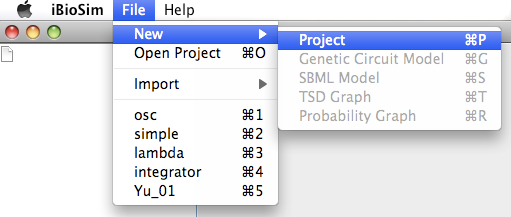
\includegraphics[height=50mm]{screenshots/project}

\item Select {\tt File} $\rightarrow$ {\tt New} $\rightarrow$ {\tt SBML Model}.
      Enter {\tt lambda} as the SBML model ID at which point an SBML
      editor will open.

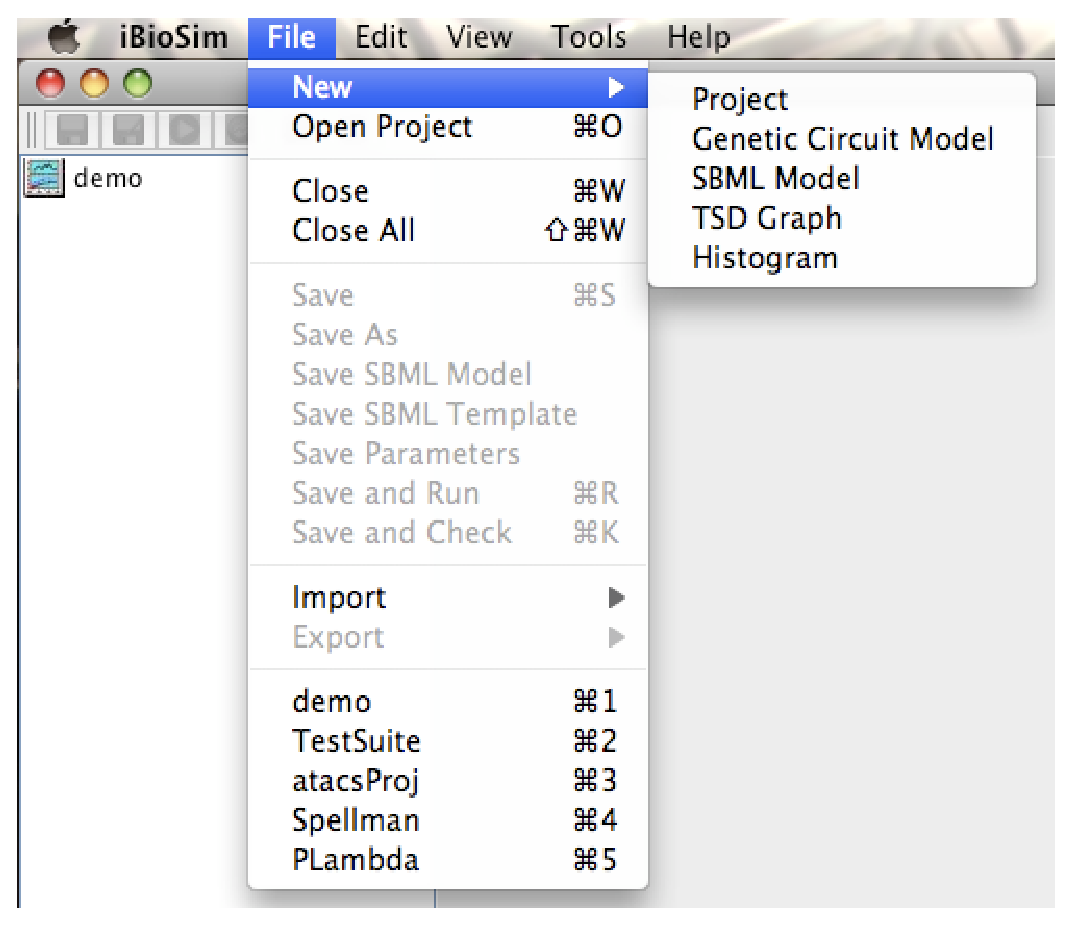
\includegraphics[height=45mm]{screenshots/newModel}

\clearpage

\item Highlight the {\tt default} compartment, select {\tt Edit
    Compartment}, and change its ID to {\tt Cytoplasm}.  Also, change 
    the units to {\tt volume}.

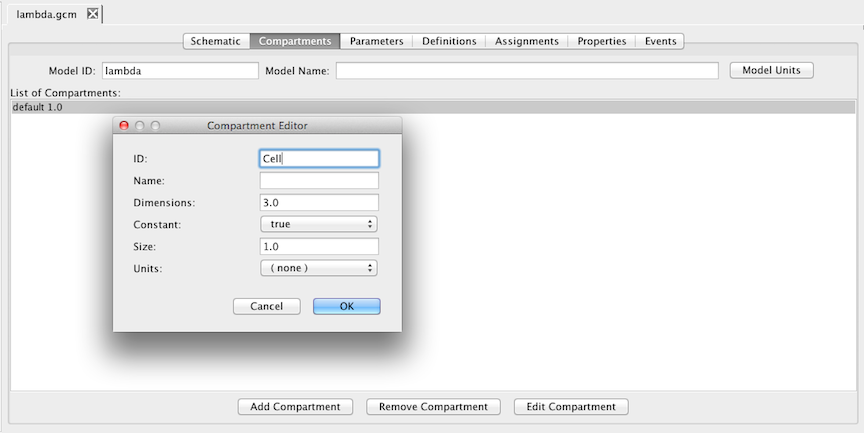
\includegraphics[height=65mm]{screenshots/compartment}

\item Select {\tt Add Species} and enter {\tt CI} as the ID, 
{\tt The lambda repressor} as the name, change the units 
to {\tt mole}, and set the {\tt Has Only Substance Units} flag to
true.  Select {\tt Add Species} again and enter {\tt CI2} as the ID,
{\tt CI dimer} as the name, change the units to {\tt mole}, and set the
{\tt Has Only Substance Units} flag to true. 

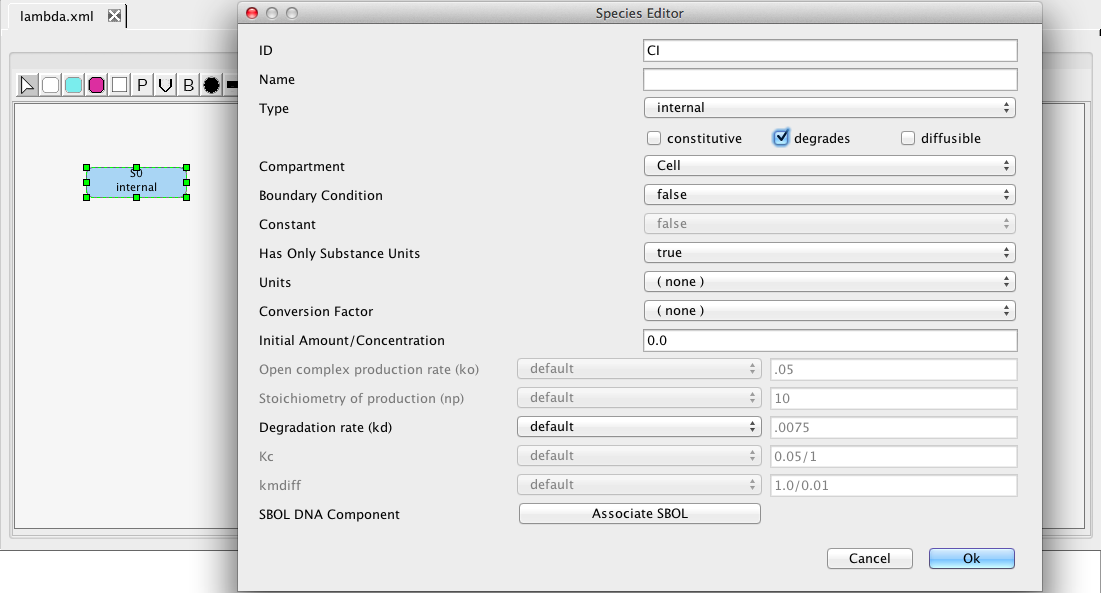
\includegraphics[height=60mm]{screenshots/species}

\item Select {\tt Add Parameter} and enter {\tt nd} as the ID,
      {\tt Number of molecules in dimer} as the name, the value to be 2,
      and change the units to {\tt dimensionless}.

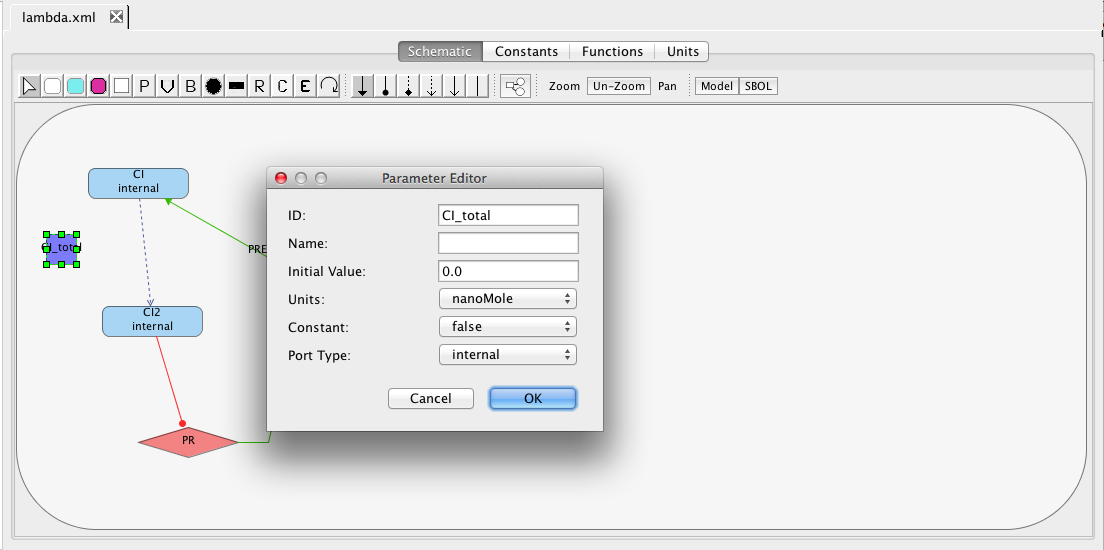
\includegraphics[height=50mm]{screenshots/parameter}

\item Select {\tt Definitions/Types} tab, and select {\tt Add Unit}
      and enter {\tt per\_second} as the ID.  Select {\tt Add to List}, 
      select {\tt second} as the kind, change the exponent to $-1$, 
      and click {\tt Add}.  Click {\tt Add} in the {\tt Unit Definition Editor}.
      Repeat these steps to create a {\tt per\_second\_mole} unit 
      (i.e., (second)$^{-1}$(mole)$^{-1}$).

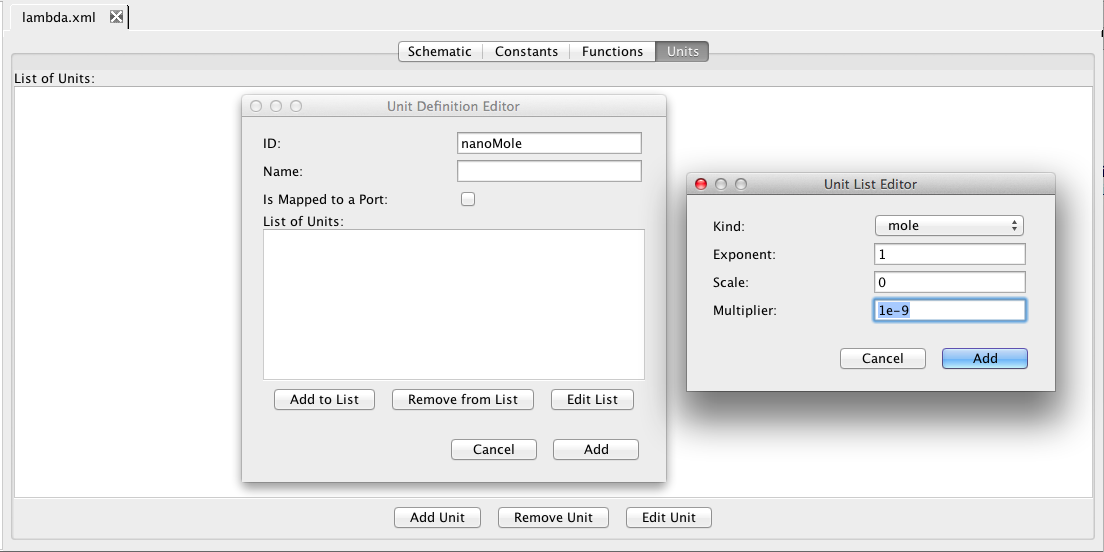
\includegraphics[height=70mm]{screenshots/units}

\item Select {\tt Main Elements} tab.  Select {\tt Add Reaction} and
  enter {\tt Dimerize\_CI} as the ID, {\tt Reaction to dimerize CI} as
  the name, and change reversible to {\tt true}.

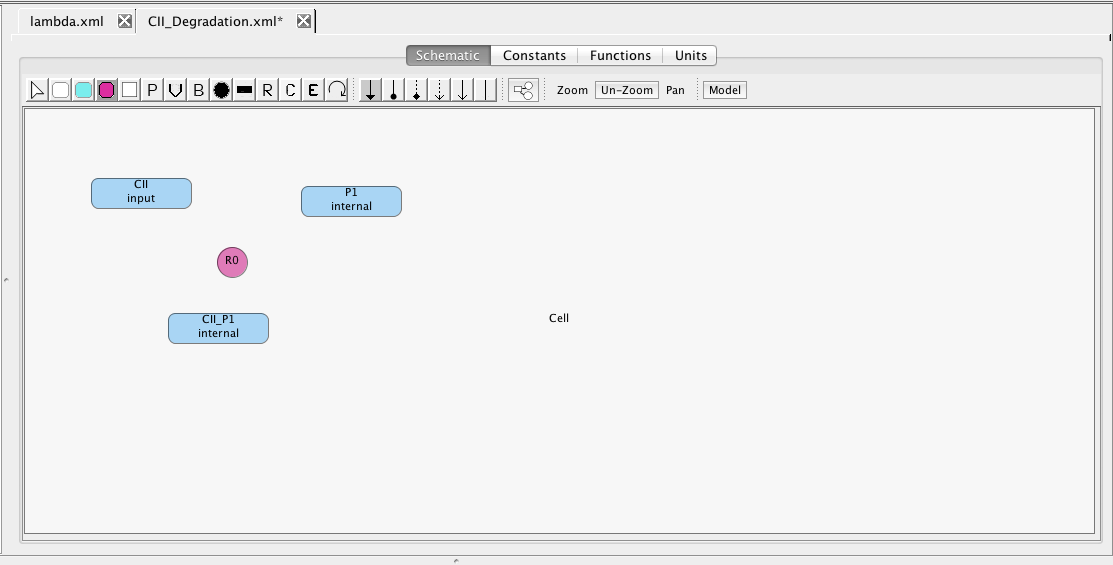
\includegraphics[height=65mm]{screenshots/reaction}

\item Select {\tt Add Reactant} and select {\tt CI} as the species,
      change {\tt Stoichiometry} to {\tt Stoichiometry math}, and set its
      value to {\tt nd}.

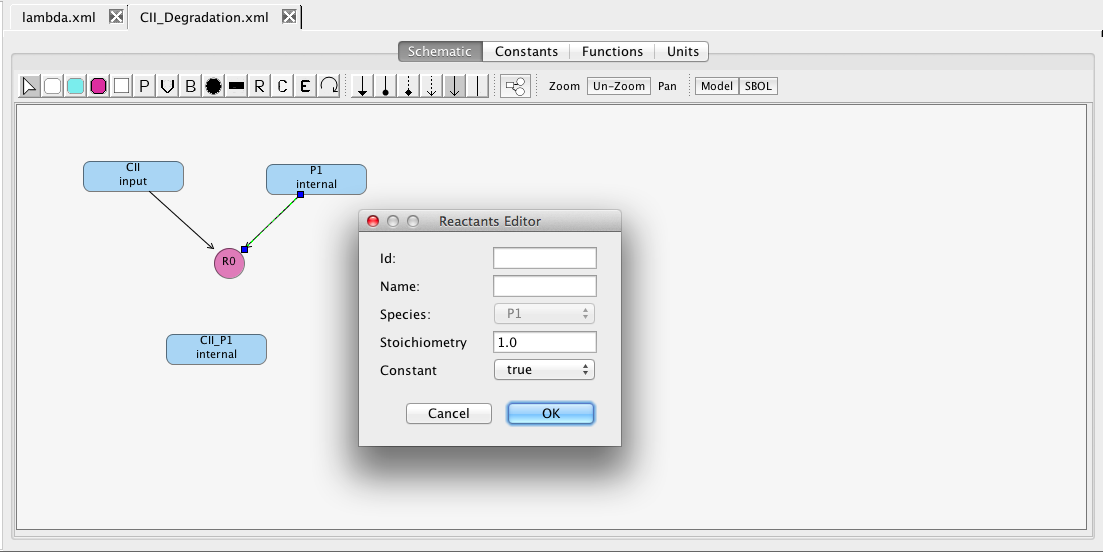
\includegraphics[height=40mm]{screenshots/reactant}

\item Select {\tt Add Product} and select {\tt CI2} as the species.
      Leave the stoichiometry as 1.

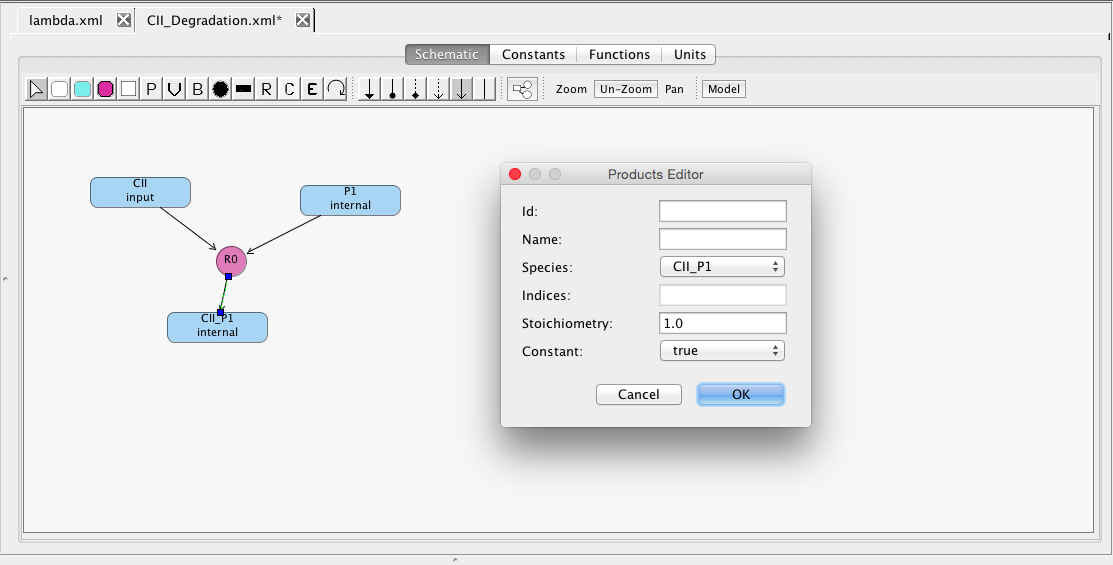
\includegraphics[height=50mm]{screenshots/product}

\item Highlight {\tt kf} and select {\tt Edit Selected Parameter}, change
      {\tt kf} to {\tt k2f}, and change the units to {\tt per\_second\_mole}.
      Highlight {\tt kr} and select {\tt Edit Selected Parameter}, change
      {\tt kr} to {\tt k2r}, and change the units to {\tt per\_second}.

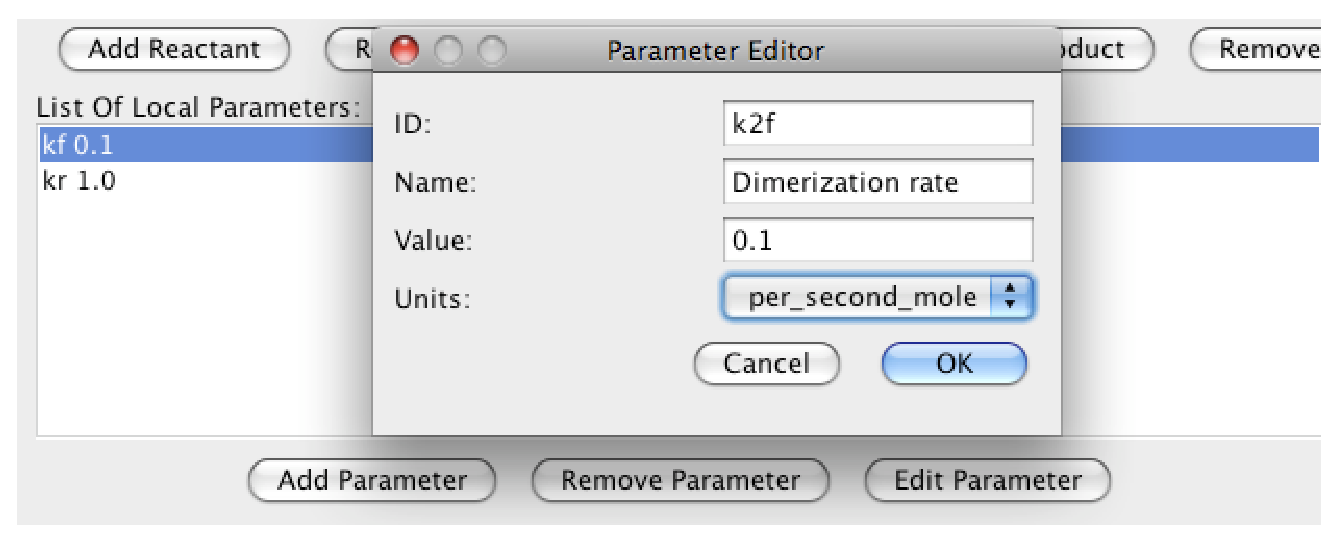
\includegraphics[height=50mm]{screenshots/localParam}

\item Select {\tt Use Mass Action}, select {\tt Add}, 
      and select {\tt Save and Check SBML}.  There should be no errors.

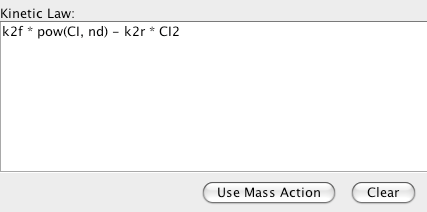
\includegraphics[height=60mm]{screenshots/kineticLaw}

\clearpage

\item Highlight {\tt lambda.sbml}, using right mouse button, select 
      {\tt View Network}.
      Highlight {\tt lambda.sbml}, using right mouse button, select 
      {\tt View in Browser}.

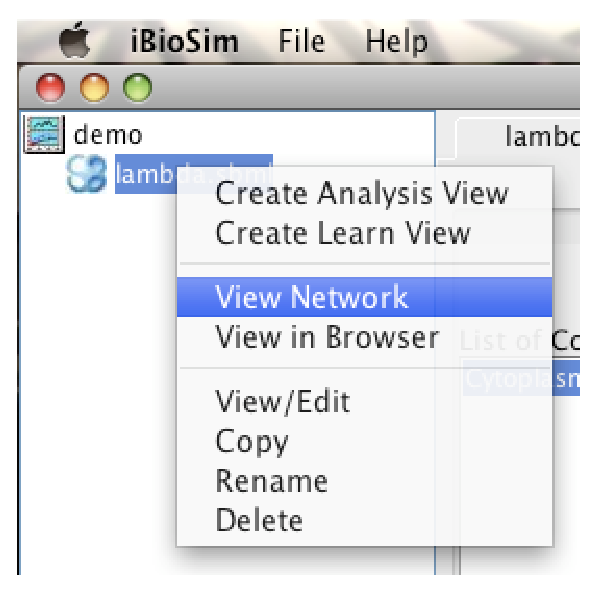
\includegraphics[height=60mm]{screenshots/viewNet}\\
\begin{tabular}{cc}
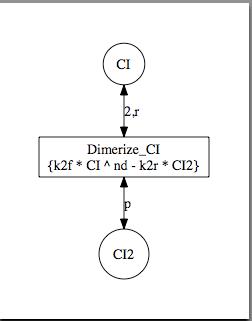
\includegraphics[height=60mm]{screenshots/viewNetwork} &
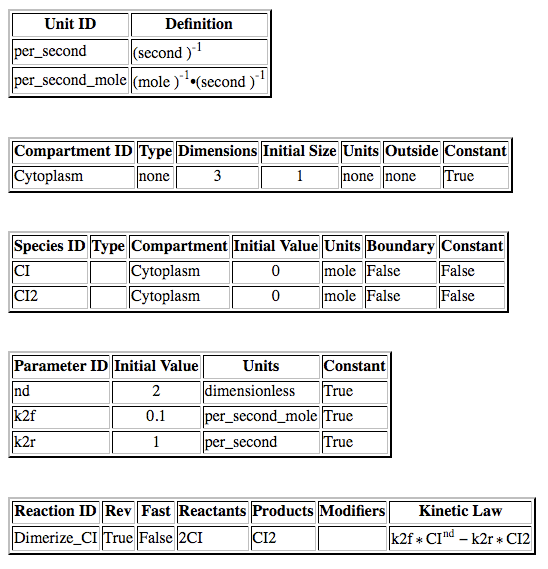
\includegraphics[height=100mm]{screenshots/viewBrowser}
\end{tabular}

\clearpage

\item Go back to the SBML editor complete the construction of the
      chemical reaction network shown below:
\begin{eqnarray*}
PRE + \mathrm{RNAP} & \stackrel{KPRE2}{\longleftrightarrow} &
PRE\_\mathrm{RNAP} \\
PRE + \mathrm{CII} + \mathrm{RNAP} &
\stackrel{KPRE4}{\longleftrightarrow} &
PRE\_\mathrm{CII}\_\mathrm{RNAP} \\
PRE\_\mathrm{RNAP} & \stackrel{kPREb}{\longrightarrow} & 
PRE\_\mathrm{RNAP} + n\mathrm{CI} \\
PRE\_\mathrm{CII}\_\mathrm{RNAP} 
& \stackrel{kPRE}{\longrightarrow} & 
PRE\_\mathrm{CII}\_\mathrm{RNAP} + n\mathrm{CI} \\
PR + \mathrm{RNAP} & \stackrel{KOR9}{\longleftrightarrow} &
PR\_\mathrm{RNAP} \\
PR + 2 \mathrm{CI2} & \stackrel{KOR10}{\longleftrightarrow} &
PR\_2 \mathrm{CI2} \\
PR\_\mathrm{RNAP} & \stackrel{kPR}{\longrightarrow} & 
PR\_\mathrm{RNAP} + n\mathrm{CII} \\
2 \mathrm{CI} & \stackrel{K2}{\longleftrightarrow} & \mathrm{CI2} \\
\mathrm{CI} & \stackrel{k1}{\longrightarrow} & () \\ 
\mathrm{CII} & \stackrel{k10}{\longrightarrow} & ()
\end{eqnarray*}

\begin{center}
\begin{math}
\begin{array}{|c|c|c|c|c|c|}
\hline
Constant & Value & Constant & Value & Constant & Value \\ \hline \hline
KPRE2  & 0.01~M^{-1} & KPRE4  & 0.00161~M^{-2} & 
kPREb  & 0.00004~\mathrm{sec}^{-1} \\ \hline
kPRE   & 0.015~\mathrm{sec}^{-1} &
KOR9  & 0.69422~M^{-1} & KOR10  & 0.06568~M^{-2} \\ \hline
kPR    & 0.014~\mathrm{sec}^{-1} &
K2       & 0.1 M^{-1} & k1       & 0.0007~\mathrm{sec}^{-1} \\ \hline
k10    & 0.002~\mathrm{sec}^{-1} & n         & 10 & ~ & ~ \\ \hline
\end{array}
\end{math} \\
Set an initial amount of 1.0 for PRE and OR, 30.0 for RNAP, and 0.0 
for the rest.
\end{center}
\end{enumerate}

% \item Add a new species ``CI\_total'' with units of {\tt mole}.
%       Click on the ``Initial Assignments/Rules/Constraints/Events'' tab
%       and press the ``Add Rule'' button.
%       Select Assignment Type, select Variable ``CI\_total'', 
%       and enter the following as the Rule:
% \begin{eqnarray*}
% & 2 * CI2 + CI &
% \end{eqnarray*}
 
% 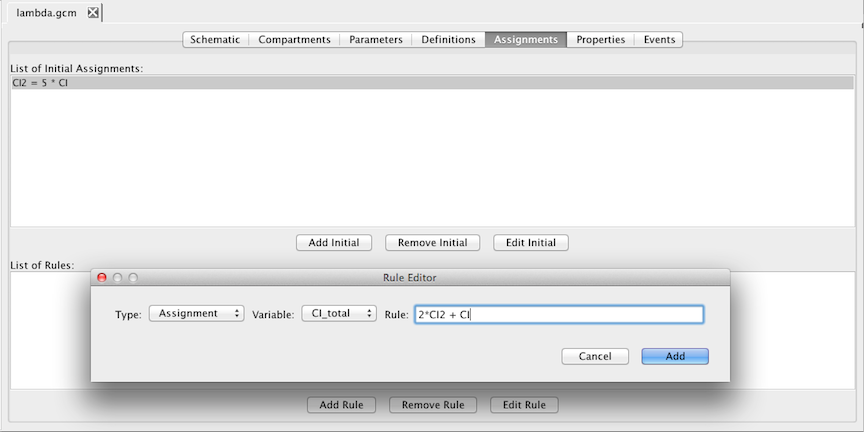
\includegraphics[height=60mm]{screenshots/rule}

\clearpage

\section{GCM Editor}

This section describes how to construct a GCM model for this example:
\begin{enumerate}
\item Select {\tt File} $\rightarrow$ {\tt New} $\rightarrow$ 
      {\tt Genetic Circuit Model}.
      Enter {\tt CI\_CII} as the GCM model ID at which point a GCM
      editor will open.

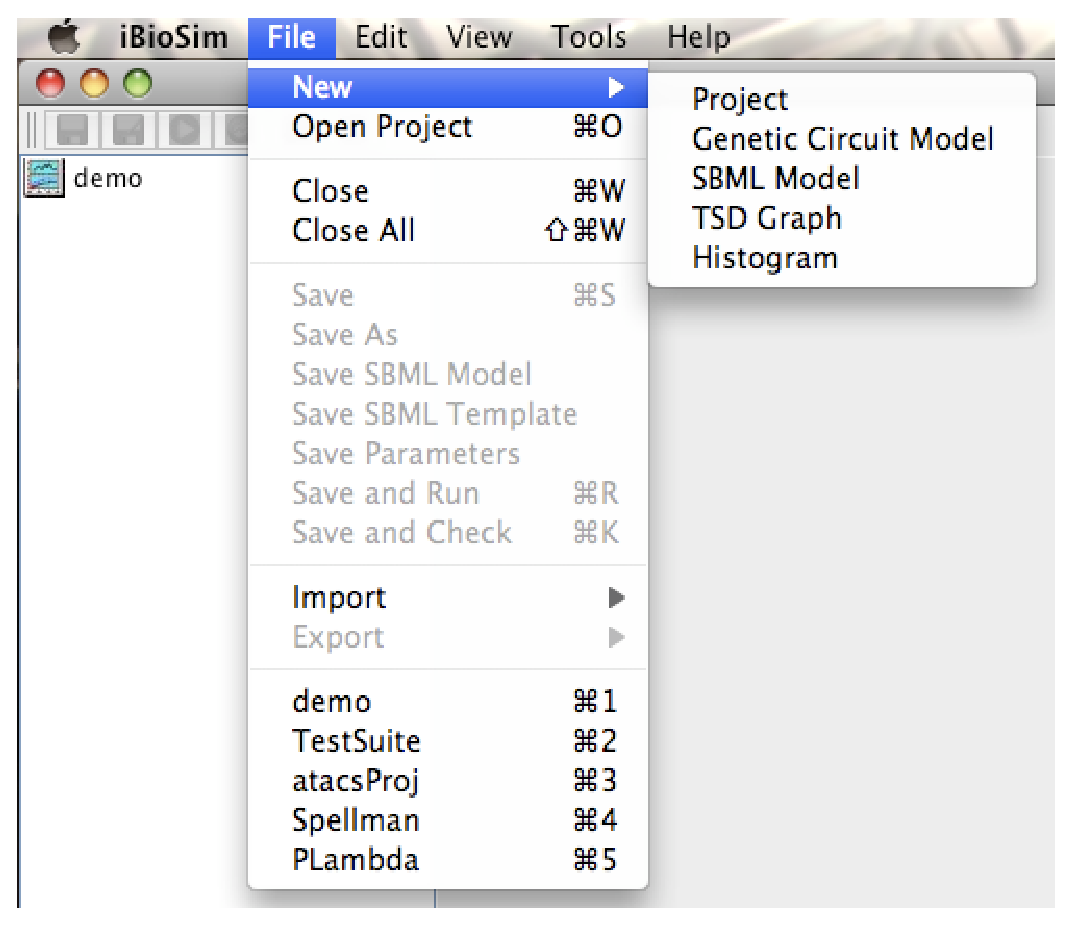
\includegraphics[height=45mm]{screenshots/newModel}

\item Select {\tt Add Promoter}, enter {\tt PR} as the ID, and press
  {\tt Ok}.  Next, add the {\tt PRE} promoter in the same way.

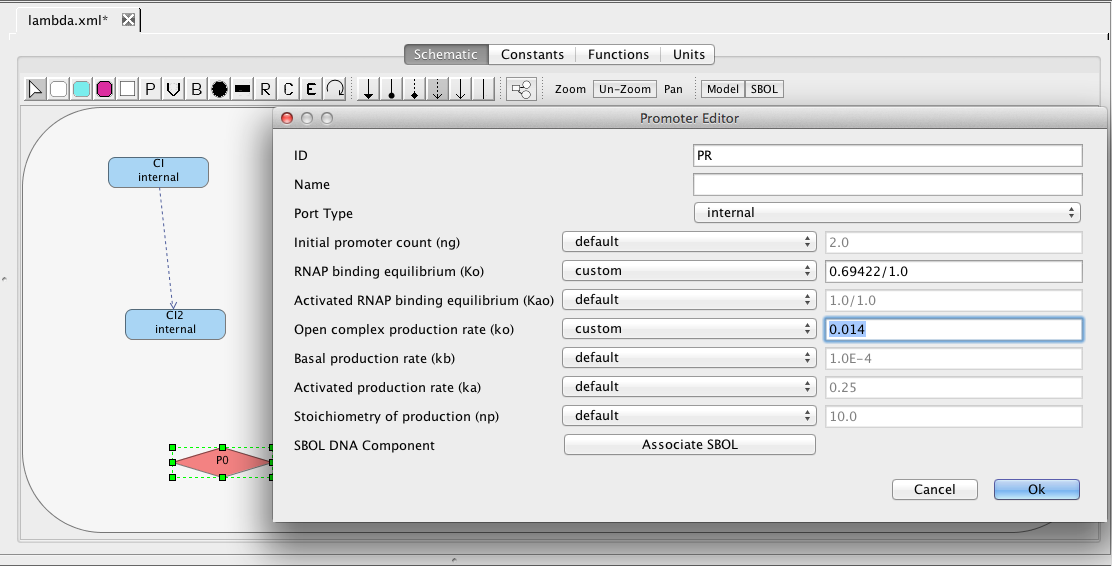
\includegraphics[height=60mm]{screenshots/promoter}

\item Select {\tt Add Species}, enter {\tt CI} as the ID, and press
  {\tt Ok}.  Next, add the {\tt CII} species in the same way.

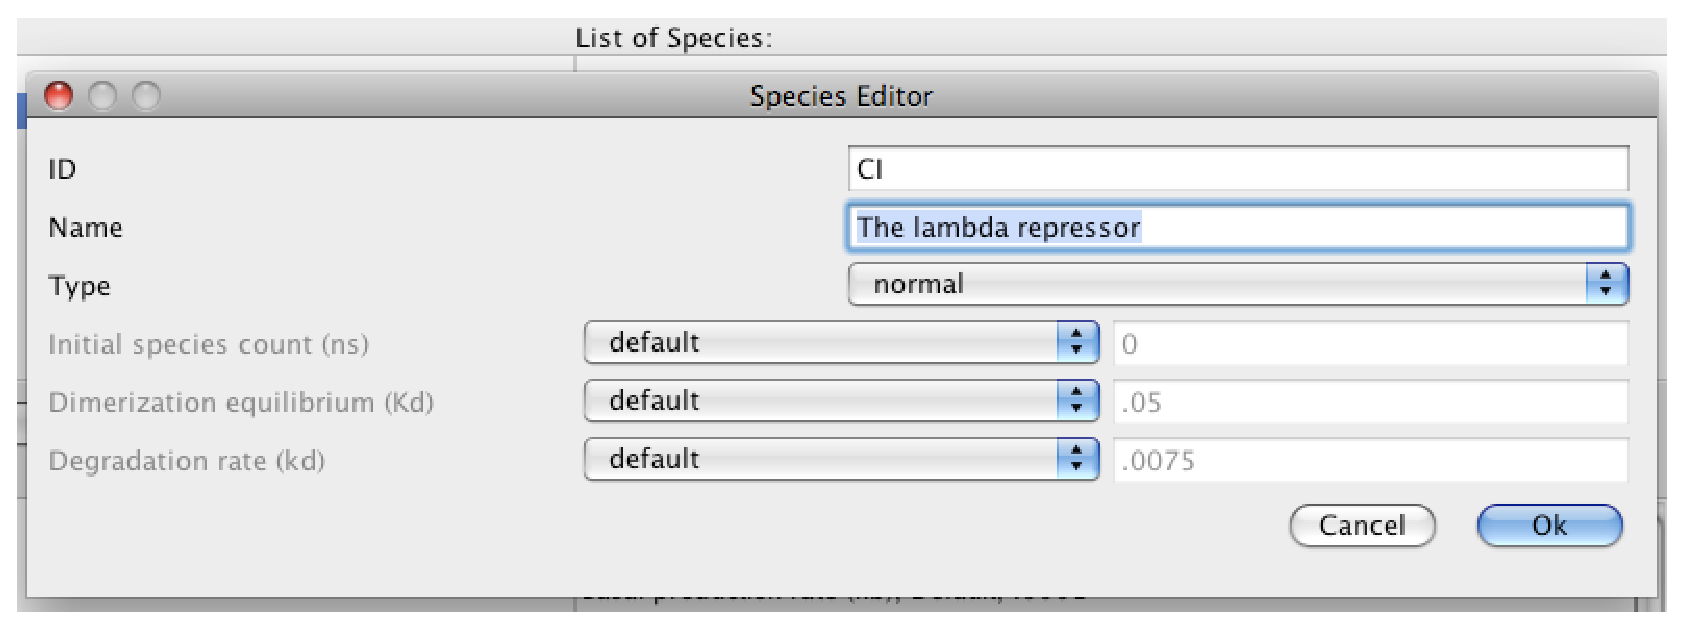
\includegraphics[height=55mm]{screenshots/GCMspecies}

\clearpage

\item Select {\tt Add Influence}, change the input to {\tt CI}, change
  the output to {\tt CII}, change the promoter to {\tt PR}, and the
  type to {\tt repression}.  Next, add an activation influence between
  {\tt CII} and {\tt CI} on promoter {\tt PRE}.

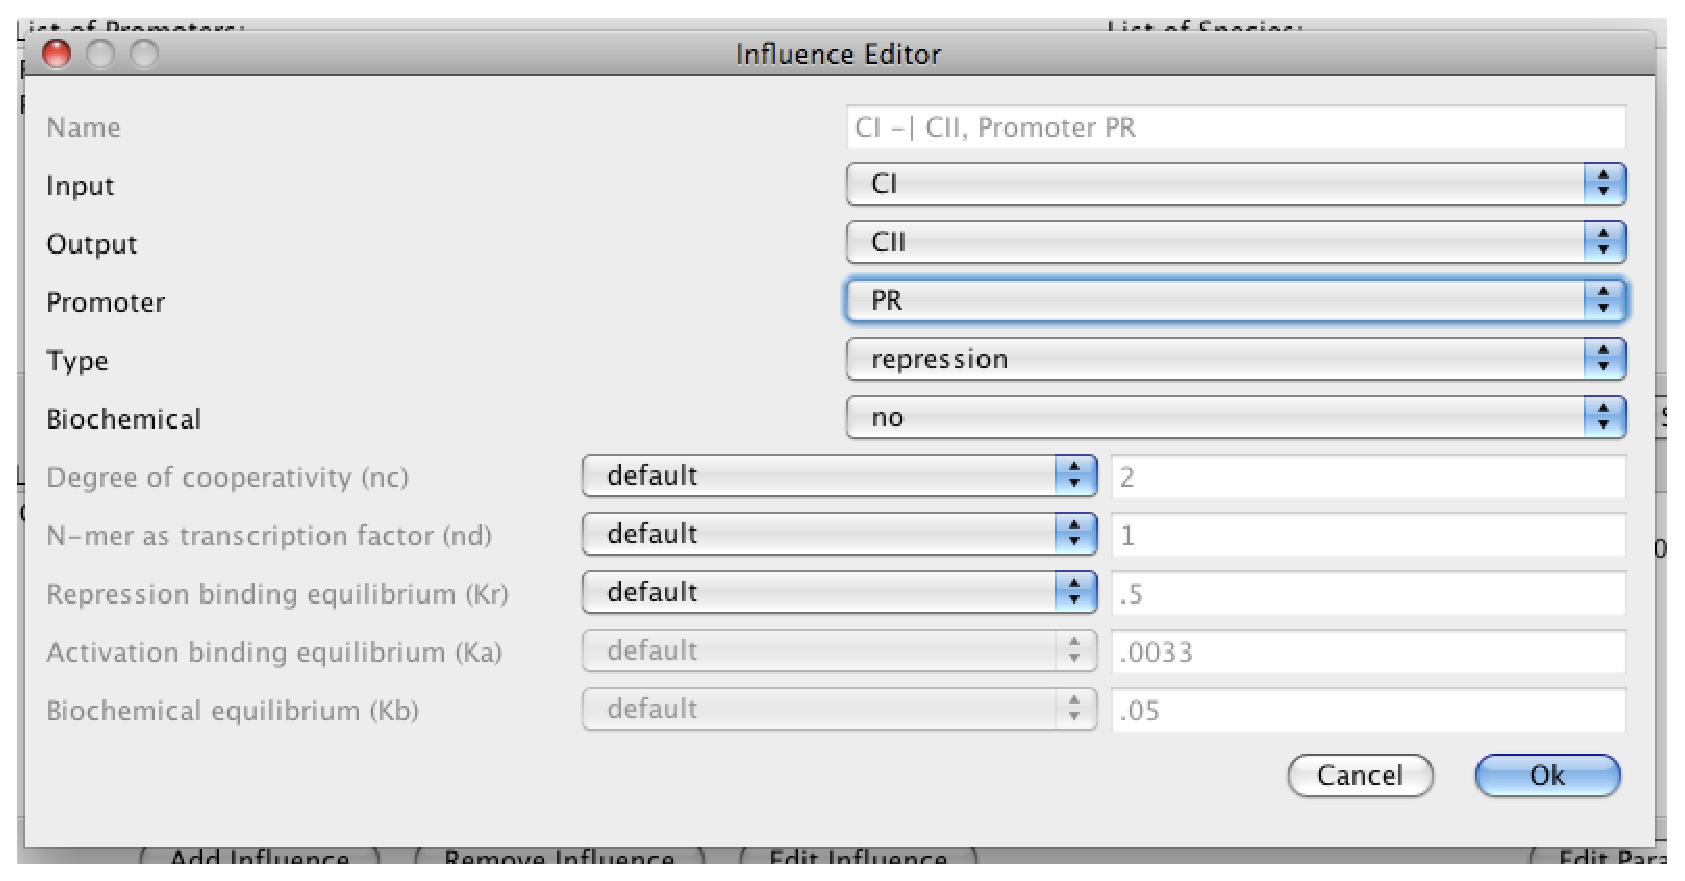
\includegraphics[height=75mm]{screenshots/influence}

\item Select {\tt Save GCM}, highlight {\tt CI\_CII.gcm} file, and
  right click to select {\tt View Genetic Circuit}.

\begin{tabular}{cc}
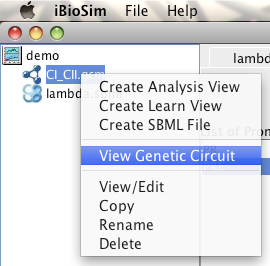
\includegraphics[height=60mm]{screenshots/viewGenNet}&
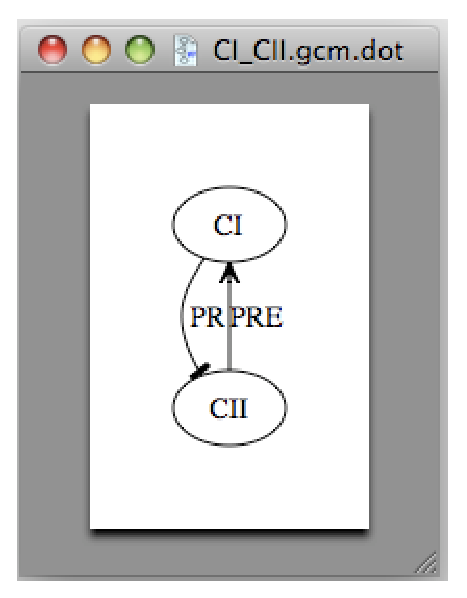
\includegraphics[height=60mm]{screenshots/viewGCM}
\end{tabular}
\end{enumerate}

\clearpage 

\section{Analysis}

The following instructions describe how to analyze the GCM file just 
created.  The SBML file can also be simulated using the following steps.  
\begin{enumerate}
\item Select {\tt Save GCM}, highlight {\tt CI\_CII.gcm} file,
  right click to select {\tt Create Analysis View}, and set the
  analysis ID to {\tt sim}.

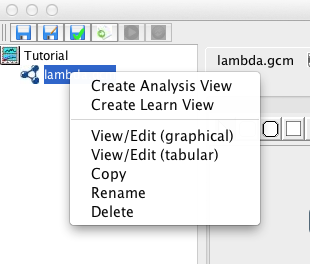
\includegraphics[height=60mm]{screenshots/GCMAnalysis}

\item In the newly opened window, select {\tt ODE}.
      Also, in this window, change the time limit to 2100.0 and print interval
      to 10.0. Finally, select {\tt Save and Run} at the bottom of the window.

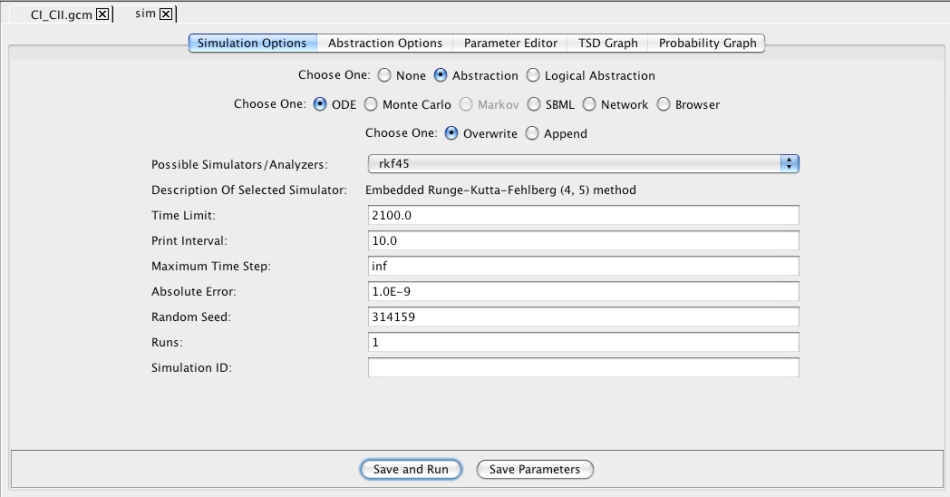
\includegraphics[height=80mm]{screenshots/analysisView}

\clearpage

\item After the simulation completes, click on the {\tt TSD Graph} tab.
%% 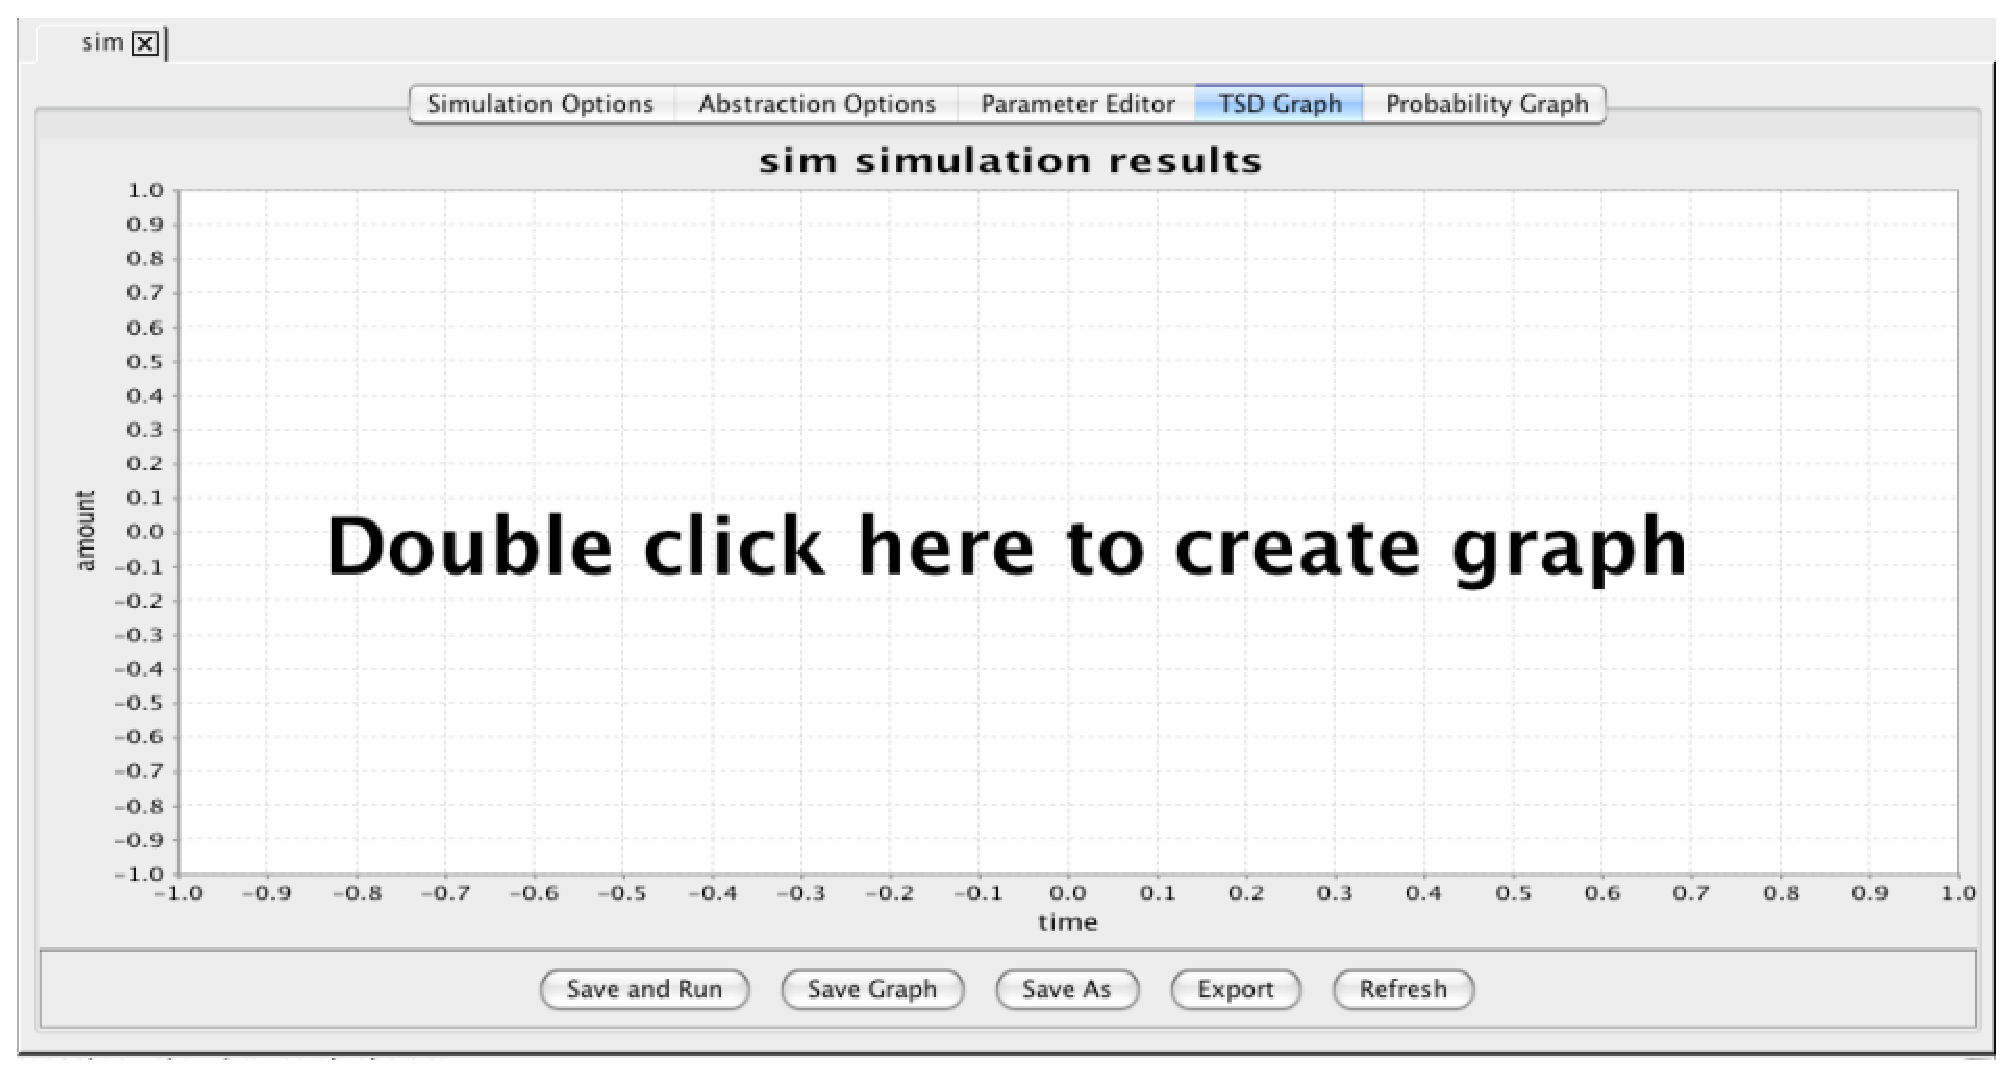
\includegraphics[height=30mm]{screenshots/emptyGraph}
%% \item 
Double click on the graph to bring up the graph editor.
  Highlight Average, if not already highlighted, select CI and CII, 
change the Title to ``ODE Simulation Results'', 
change the X-Axis Label to ``Time
(seconds)'', and change the Y-Axis Label to ``Number of Molecules''.  
Press the OK button.  Click on Export and enter file name of {\tt ode.jpg}.

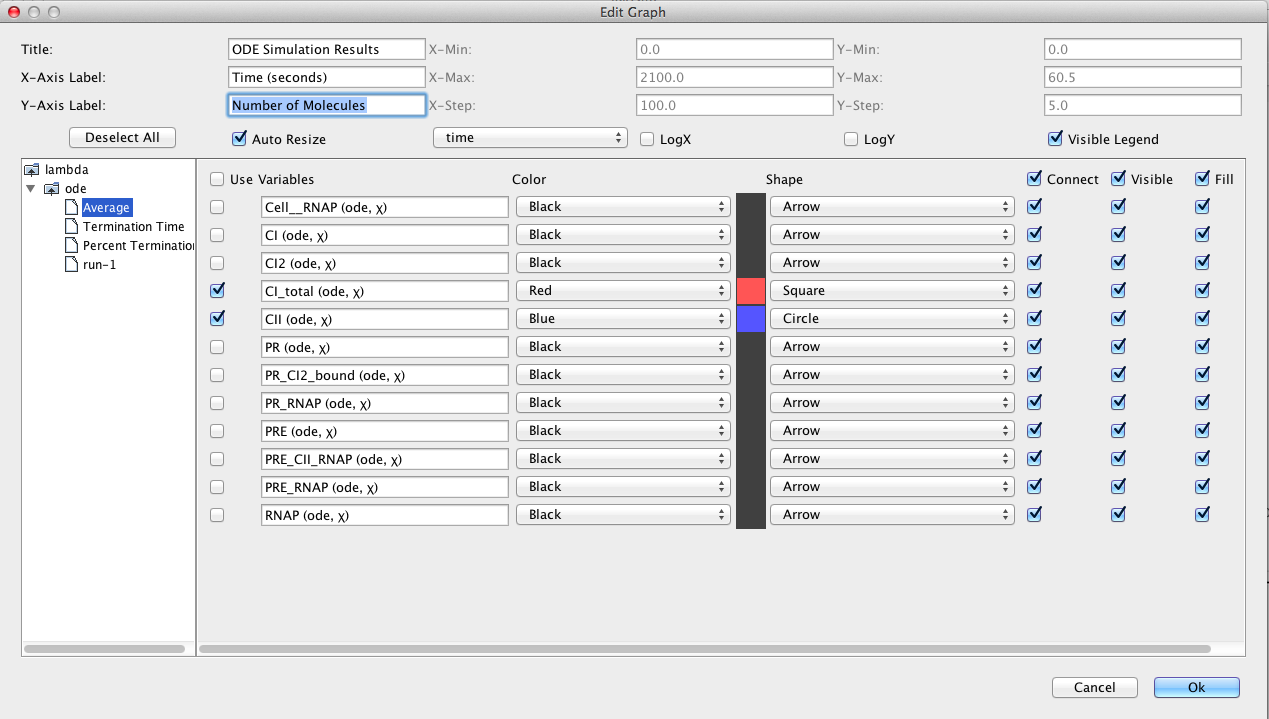
\includegraphics[height=80mm]{screenshots/odeResults}\\
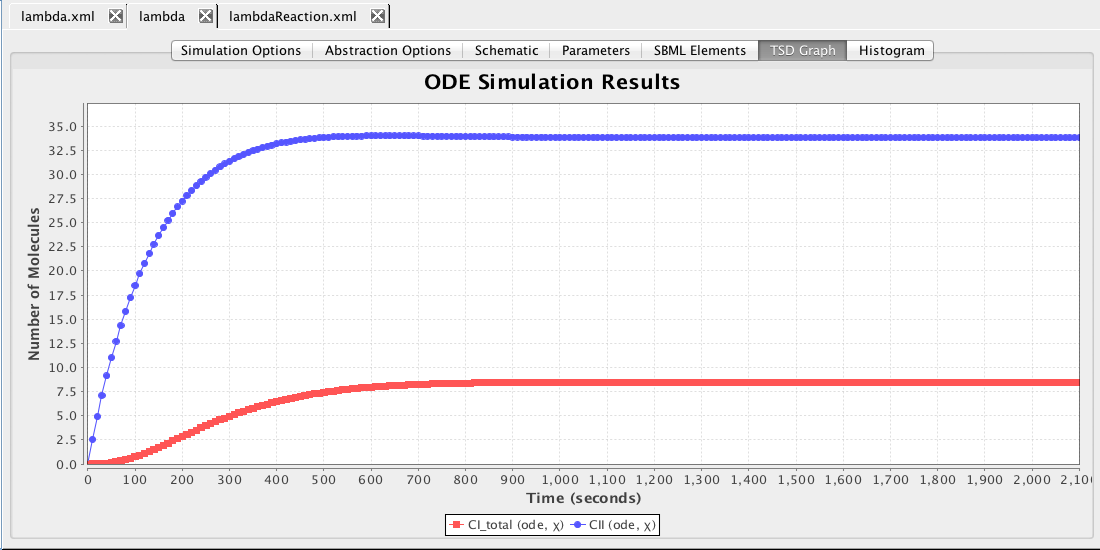
\includegraphics[height=90mm]{screenshots/odeSimResults}

\clearpage

\item Select the simulation options tab again, select {\tt Monte
    Carlo}, change the number of runs to 100, and set the simulation ID
  to {\tt ssa}.  Click on {\tt Save and Run}.  Click on the {\tt TSD
    Graph} tab.
Double click on the graph to bring up the graph editor.
Open the ssa simulation directory, and highlight {\tt run-1}.
Select CI and CII, change Title to ``SSA Simulation Results'', 
change the X-Axis Label to ``Time (seconds)'', and change the Y-Axis
Label to ``Number of Molecules''.  Press the OK button.  Click on
Export and enter file name of {\tt ssa-1.jpg}.
Repeat these steps to generate graphs for the average ({\tt
  average.jpg}) and standard deviation ({\tt stddev.jpg}).
Note that you can use the ``Deselect All'' button to
remove all items from the graph.

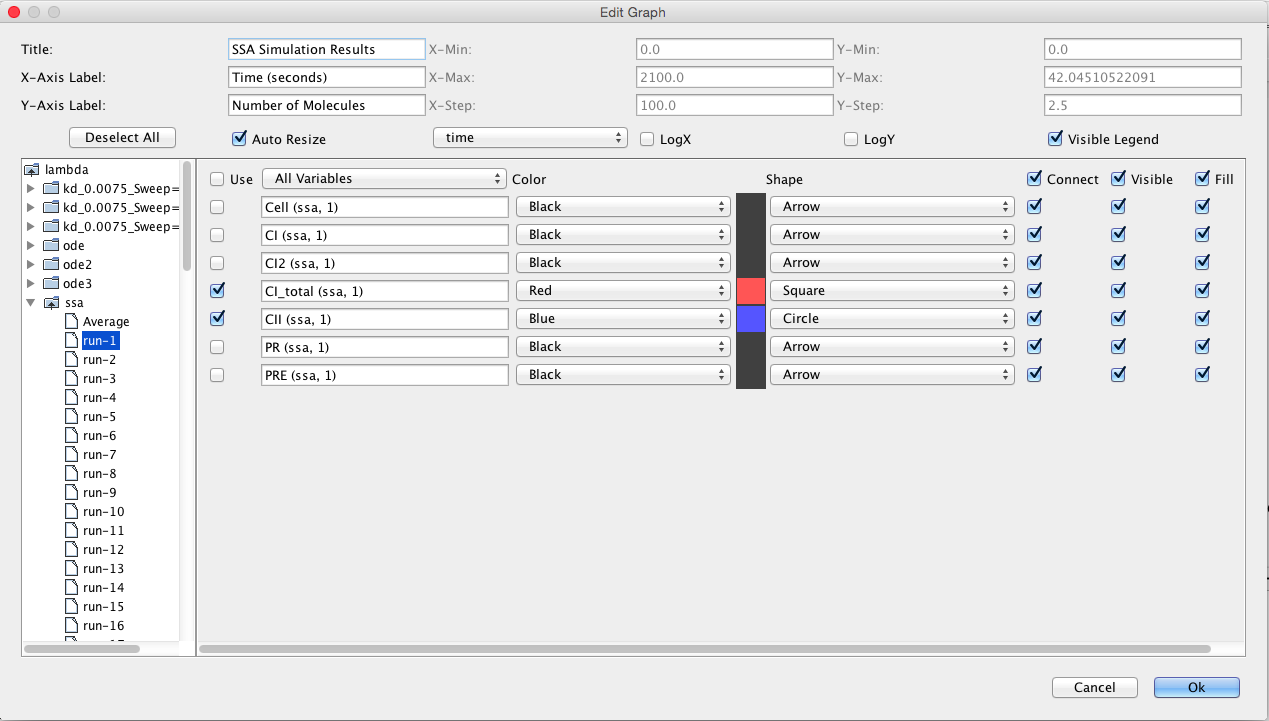
\includegraphics[height=80mm]{screenshots/ssaResults}\\
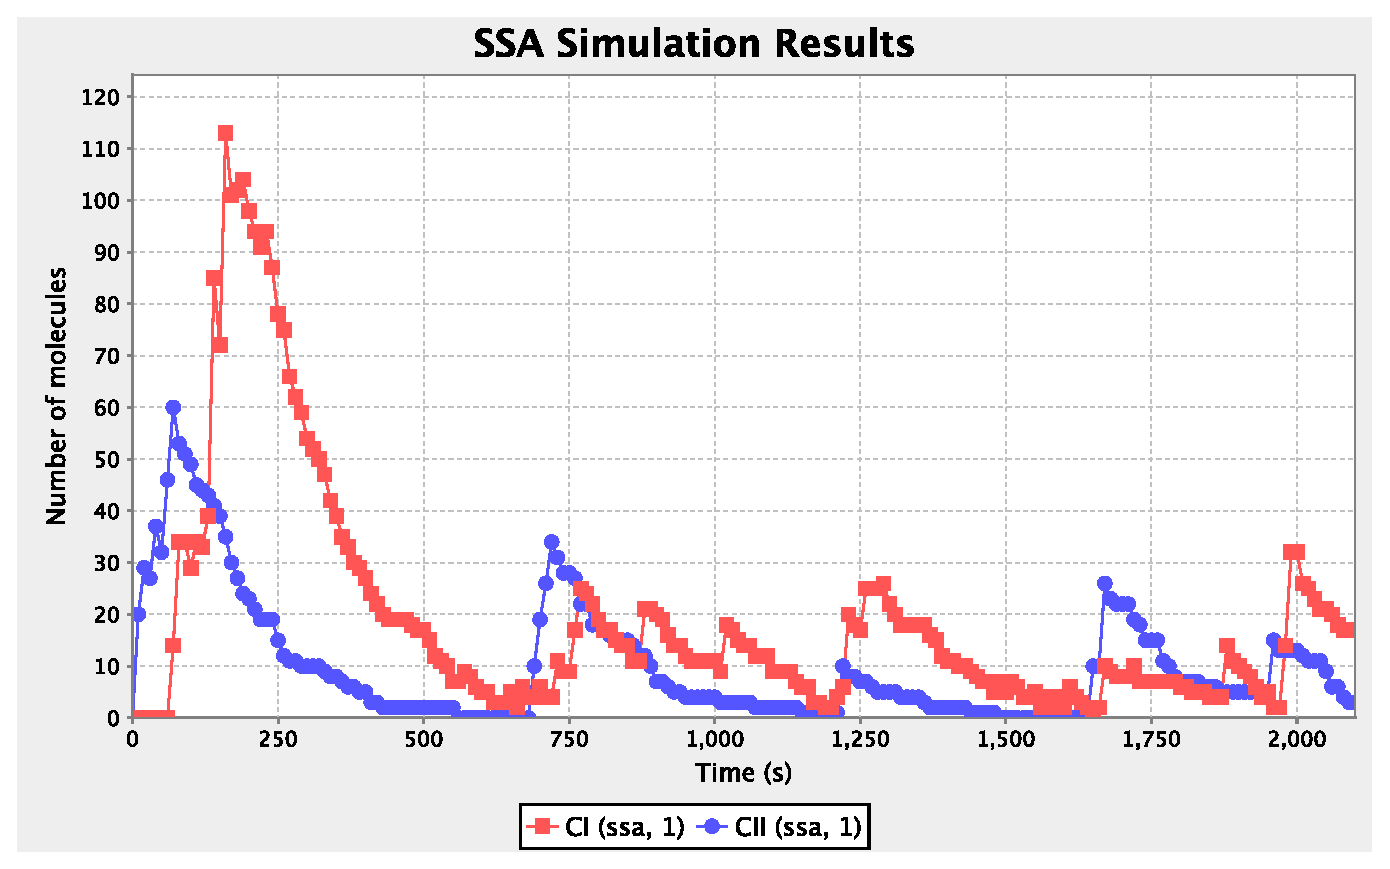
\includegraphics[height=90mm]{screenshots/ssaSimResults}

\clearpage

\item Click on the parameter editor tab.  Highlight the {\tt PR} 
      species, and select {\tt Edit Species}.  Select {\tt Custom} for
      the initial amount of {\tt PR} and change it to 5.  
      Click on the simulation options tab and change the simulation ID to
      {\tt ssa5}.
      Press the Save and Run button.
      Click on the {\tt TSD Graph} tab and following the steps above, 
      create the 
      following plots {\tt ssa-1\_5.jpg}, {\tt average\_5.jpg}, and
      {\tt stddev\_5.jpg}.  

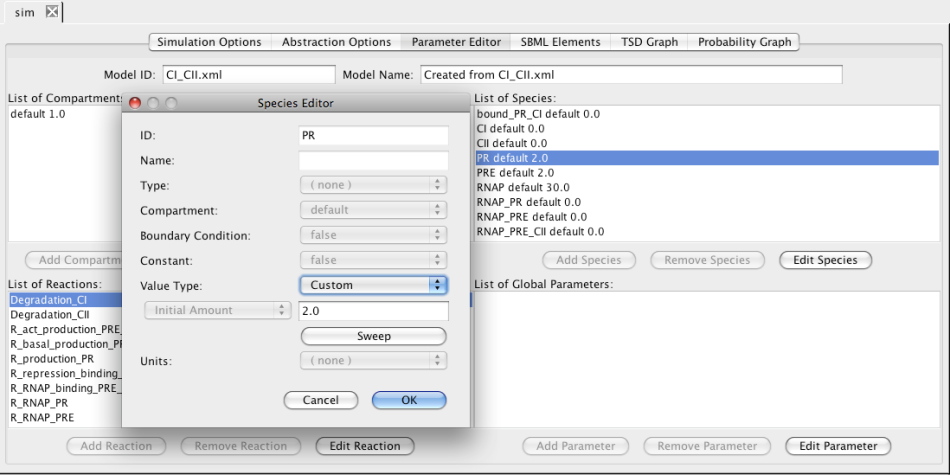
\includegraphics[height=70mm]{screenshots/paramEdit}\\
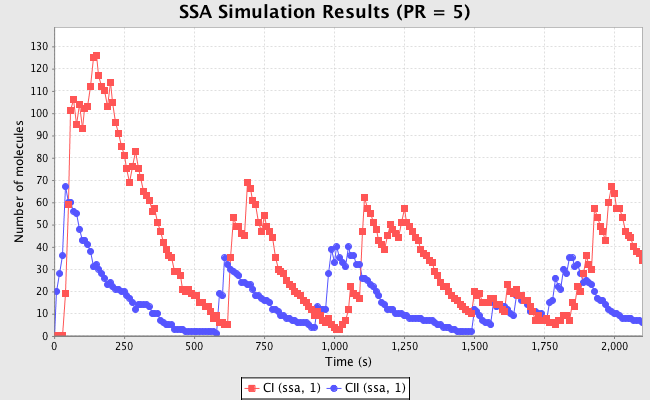
\includegraphics[height=90mm]{screenshots/ssaSimResults5}

\clearpage

\item Now go back to the parameter editor tab, 
      and change the initial amount for {\tt PR} to {\tt Sweep}, set
      the start to 2, stop to 8, step to 3.  Press the save and run
      button.  Click on the {\tt TSD Graph} tab and double click on the graph to
      open the graph editor.  Notice the new simulations id's
      generated for each of the run with PR of 2, PR of 5, and PR of
      8.  Deselect all from the current graph, and go and add the 
      average value of {\tt CI} from each of these simulation runs. 

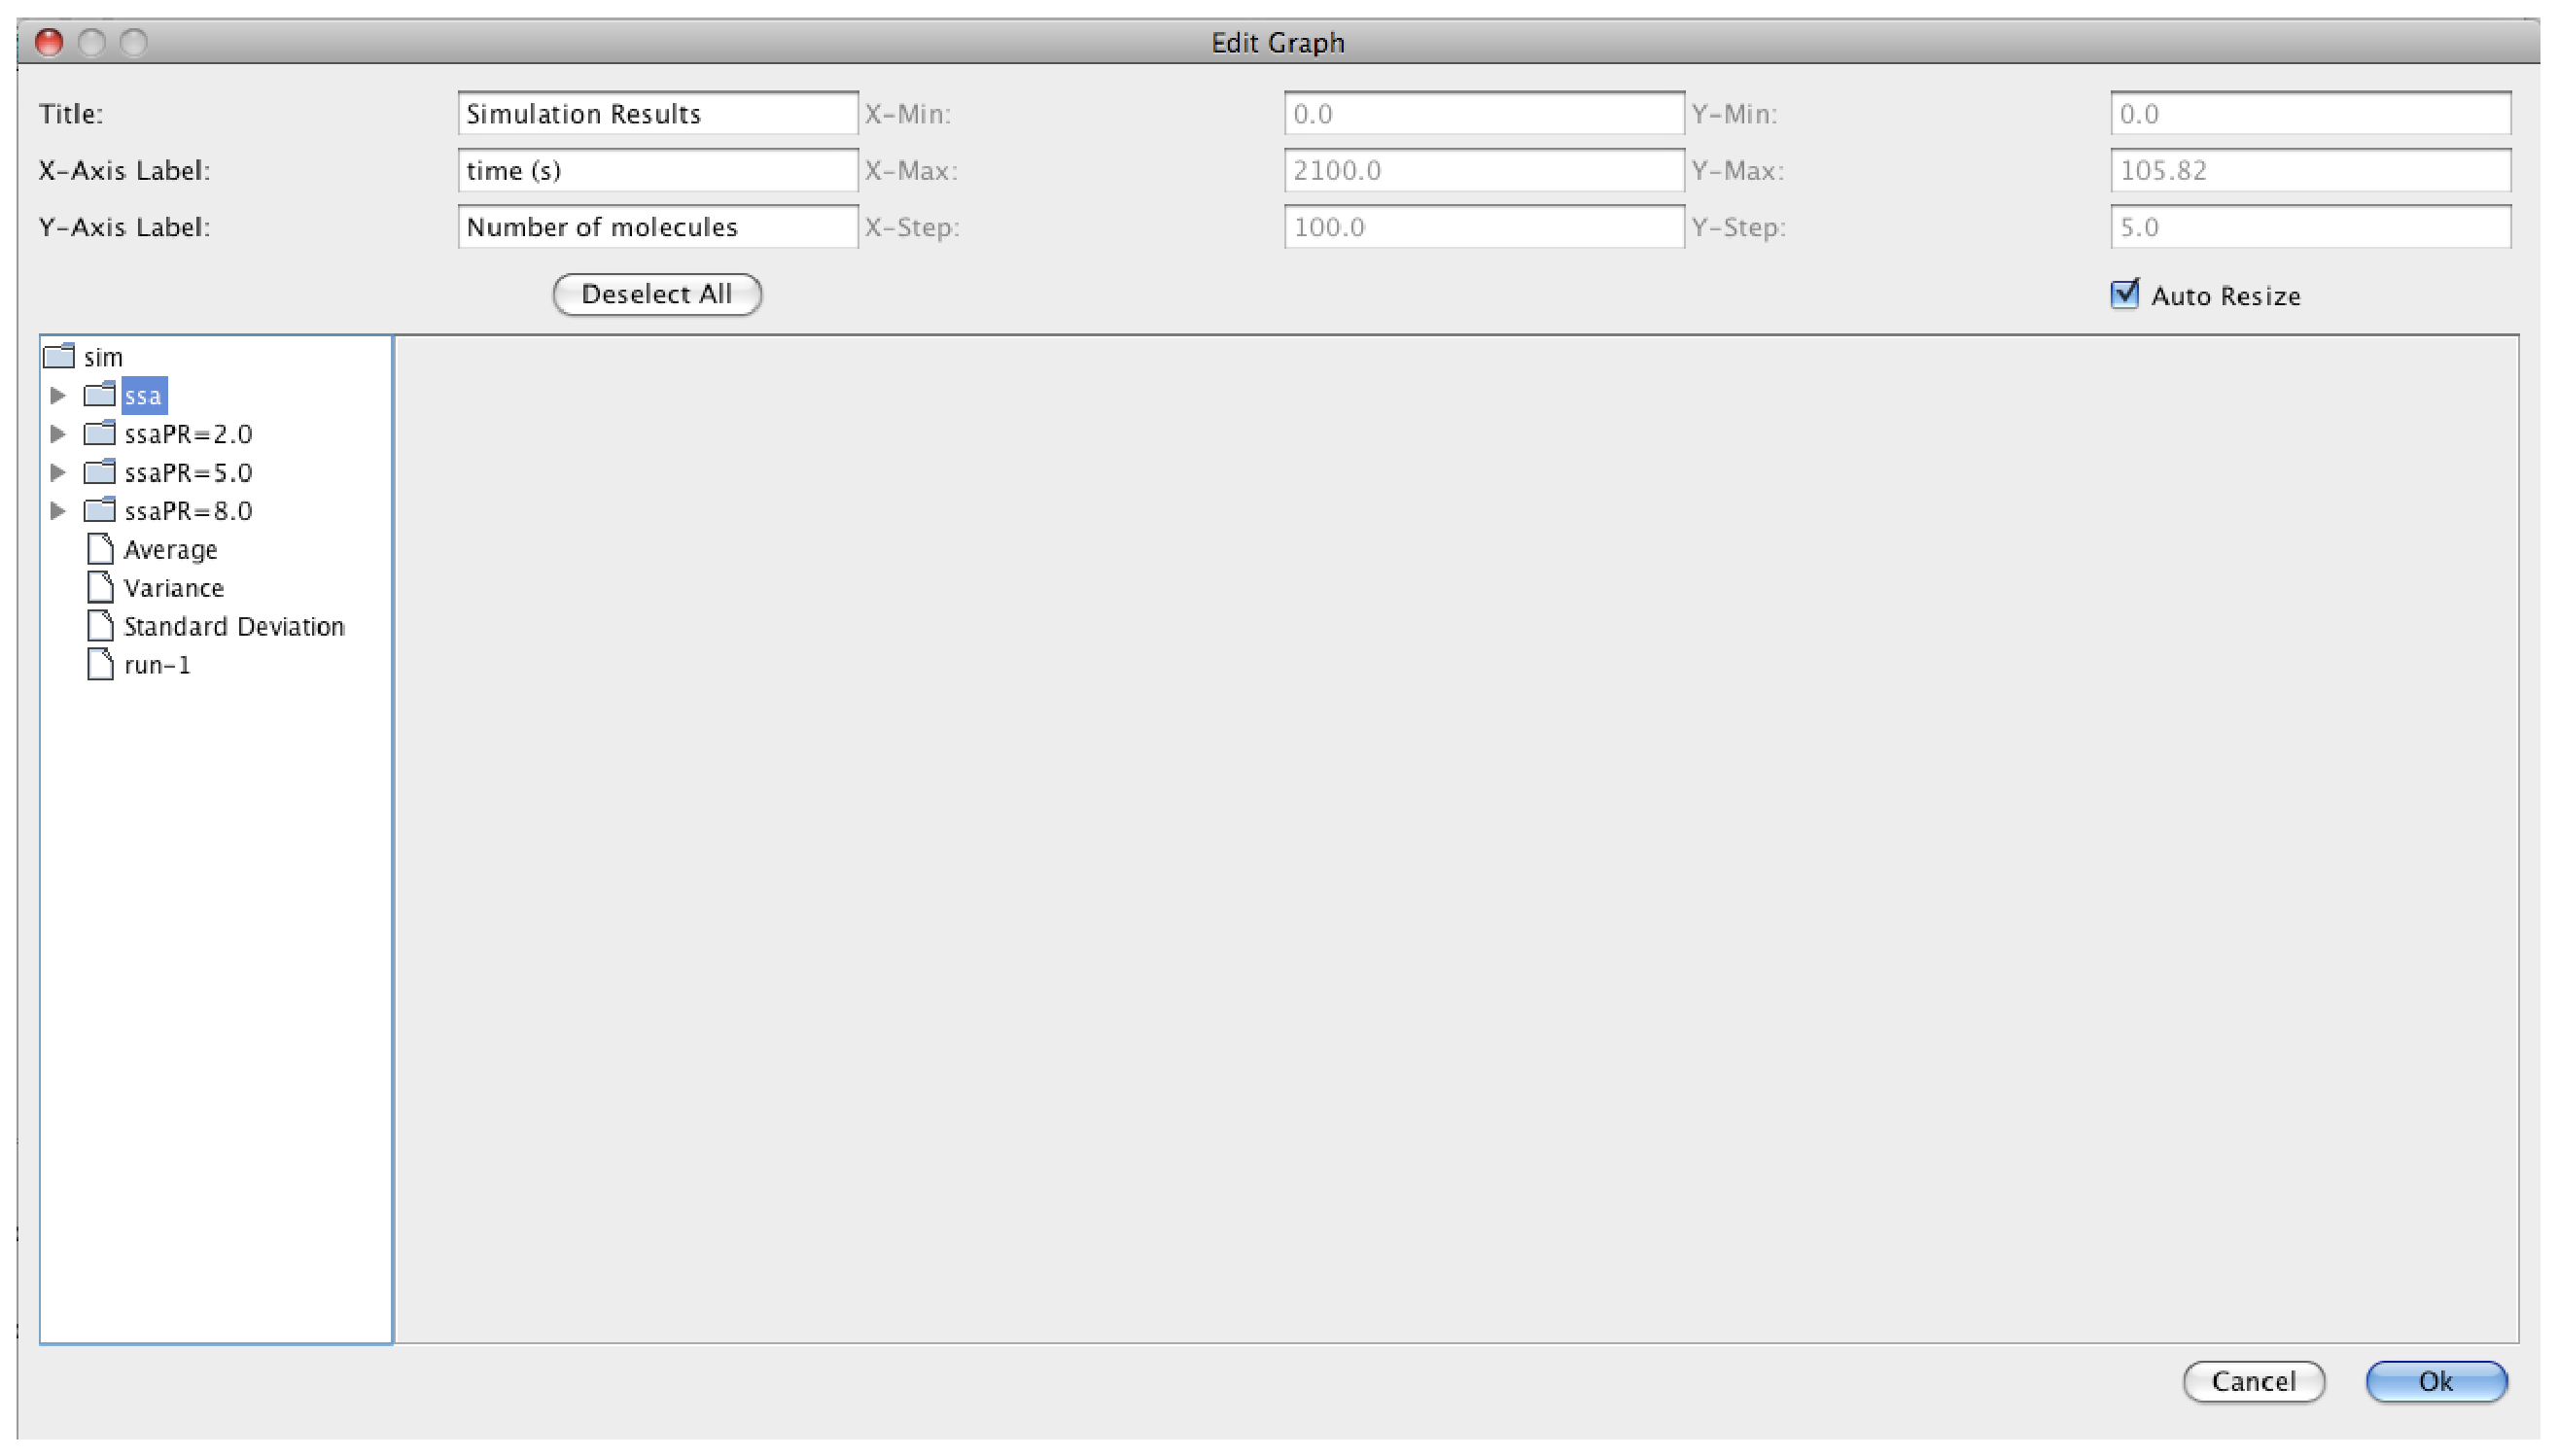
\includegraphics[height=80mm]{screenshots/sweep}\\
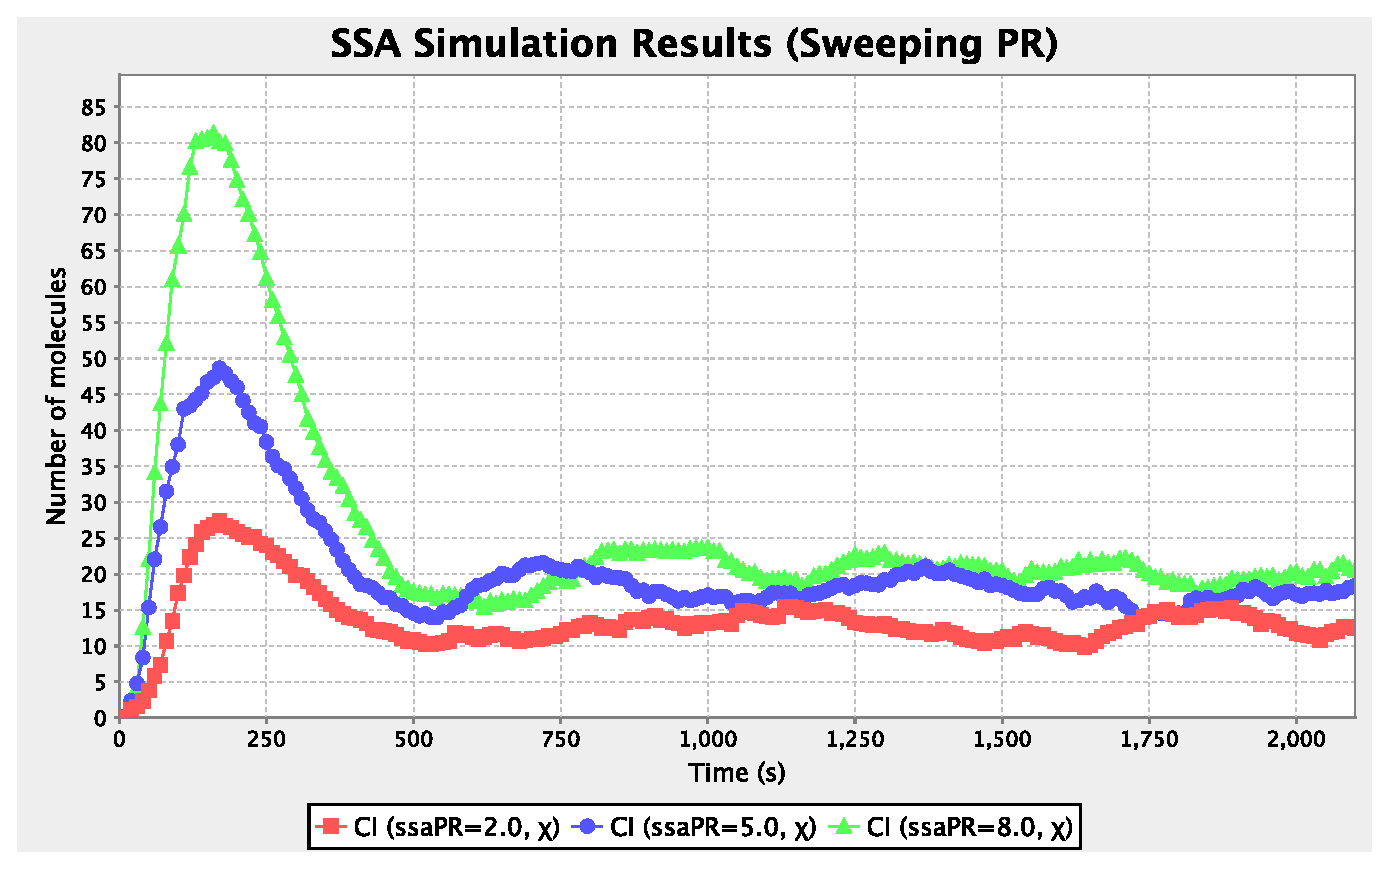
\includegraphics[height=90mm]{screenshots/sweepPR}

% \item Simulate your lambda model with BioSim using the ODE method rkf45 with
%       a time limit of 2100 and print interval of 50.
%       Make a note of the simulation time and plot CI2 and CII.  
%       Next, simulate using the Euler method.  Make a note of the simulation time
%       and add CI2 and CII from the euler results to your graph.  
%       How do the simulation times and results compare?
%       Change the time step and rerun the Euler method.  Repeat until the results
%       match up well.  What time step is required for a good match?
%       How do the simulation times compare?

\clearpage

\item Go back to the Parameter Editor tab and change {\tt PR} back to 
{\tt Original} value type.  Go back to the Simulation Options tab,
select {\tt Abstraction} and change the simulation ID to {\tt abs}.
Press {\tt Save and Run} and note that the simulation time should be
substantially faster.
Go back to the {\tt TSD Graph} tab and double click on the graph to bring up
the graph editor.  Deselect all and add the average value of {\tt CI}
from both the {\tt abs} and {\tt ssa} simulations.  
\end{enumerate}

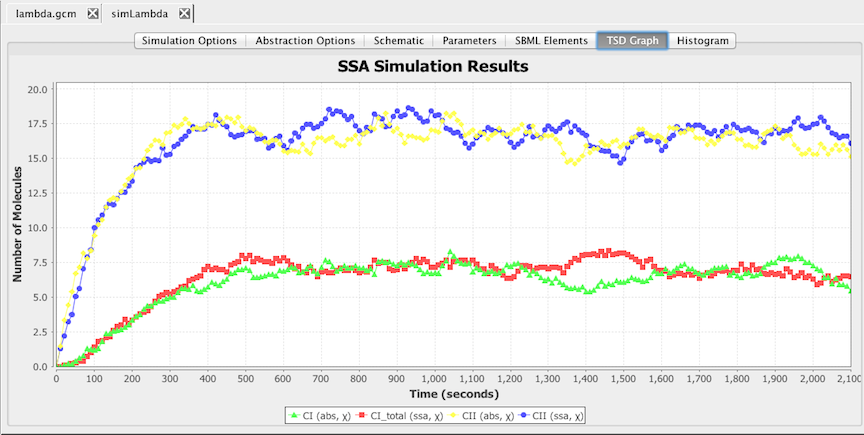
\includegraphics[height=90mm]{screenshots/absResults}

\clearpage 

\section{Probabilistic Analysis}

This example illustrates how {\tt iBioSim} can be used for
probabilistic analysis.
\begin{enumerate}
\item Go back to the GCM editor for {\tt CI\_CII}.  
Select {\tt Save as SBML Template} and give it the name {\tt
  CI\_CIIenv}.  Use the {\tt SBML File} pulldown menu to select
{\tt CI\_CIIenv.sbml} to associate with this GCM.  Press the
{\tt Save GCM} button.

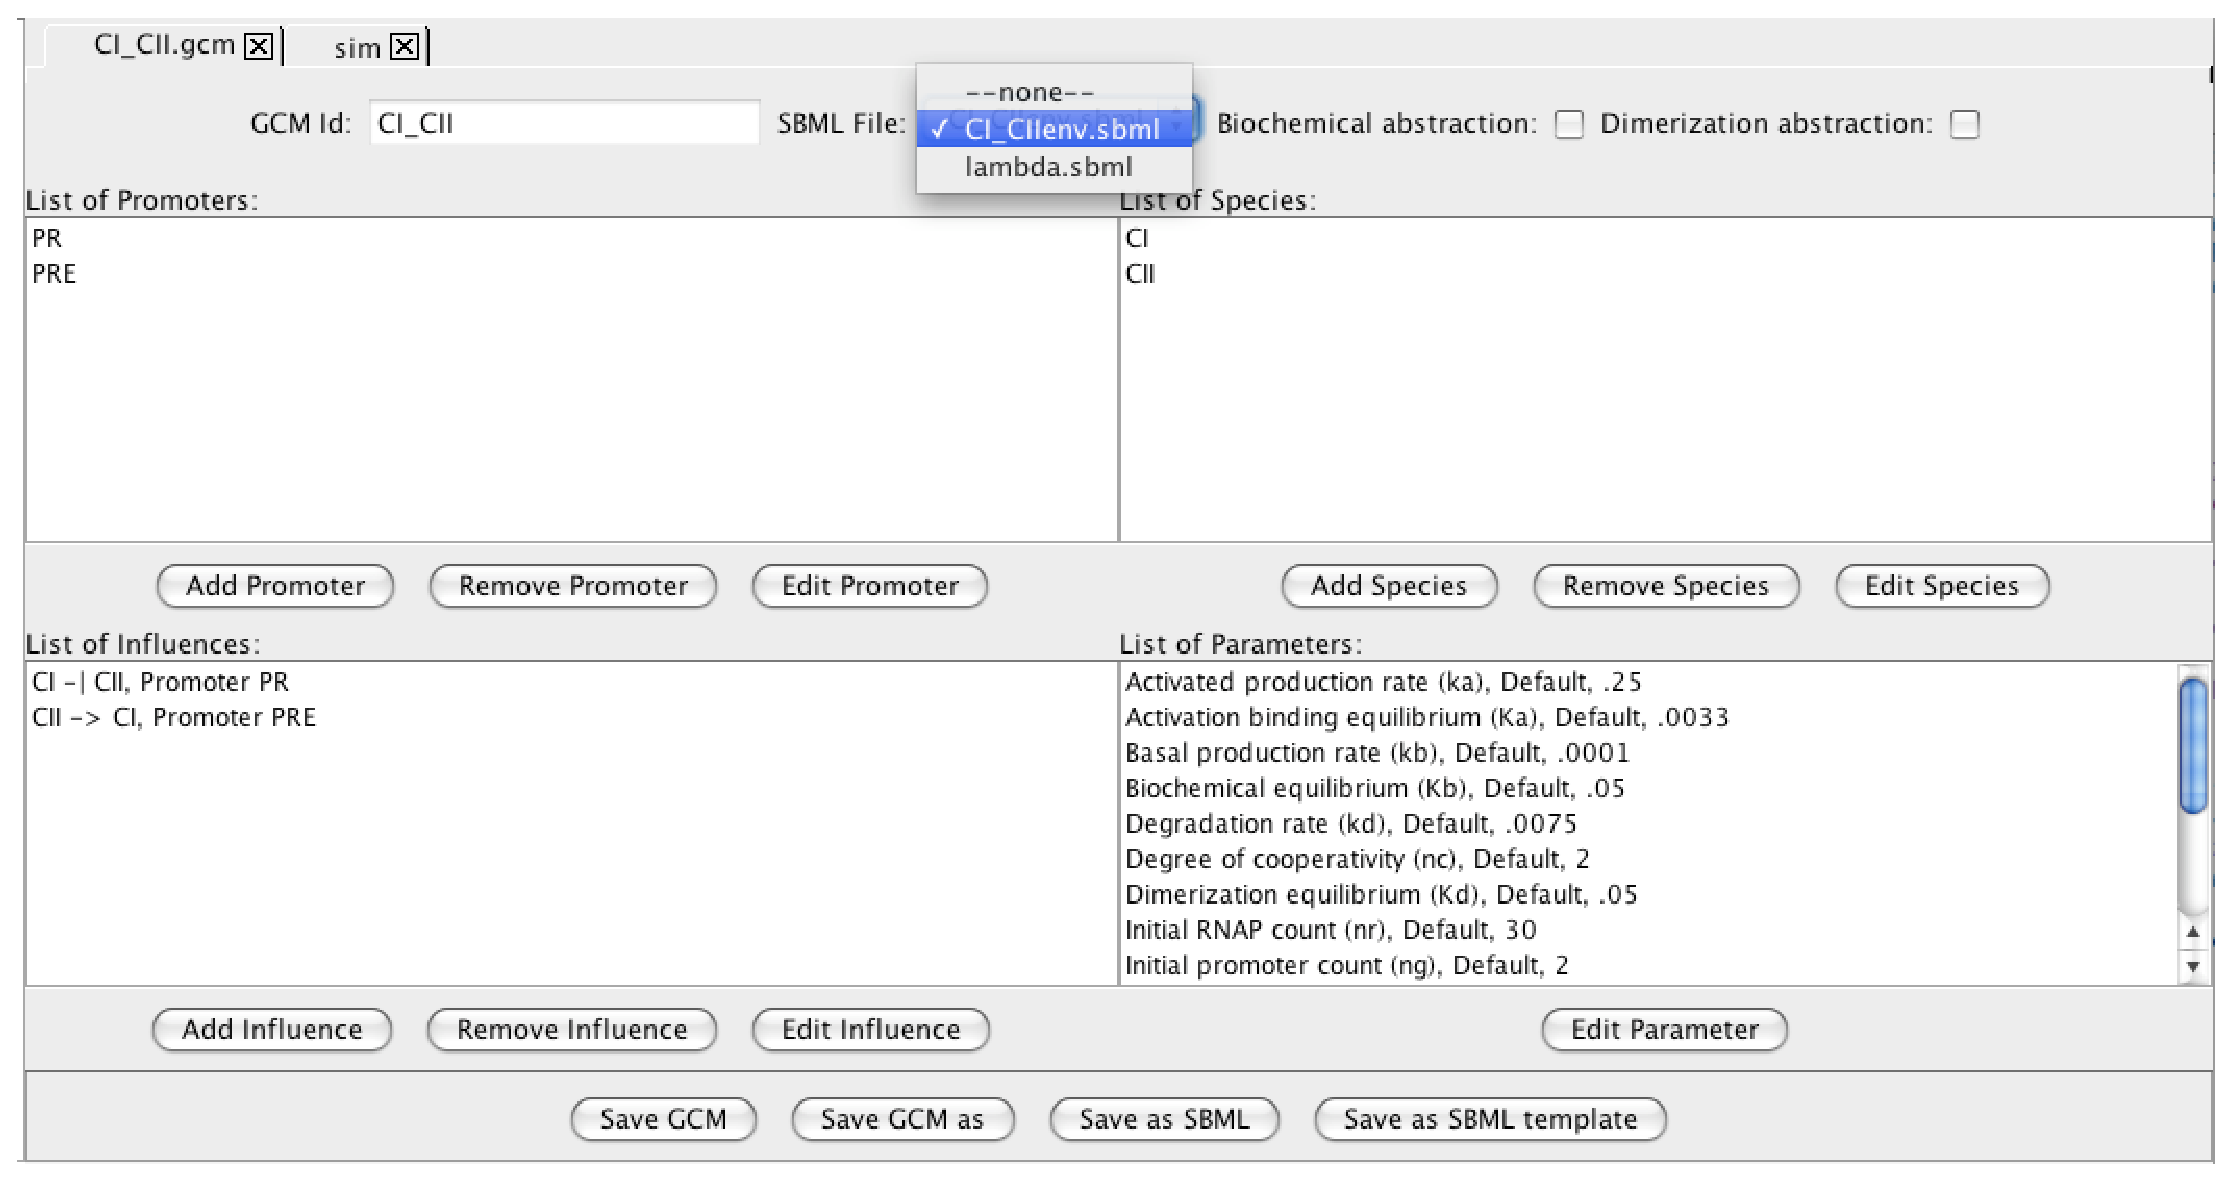
\includegraphics[height=80mm]{screenshots/linkSBML}

\item Double click on the {\tt CI\_CIIenv.sbml} file to open it in an
  SBML editor.  Select the {\tt Initial
    Assignments/Rules/Constraints/Events} tab, and select {\tt Add
    Constraint}.  Add a constraint with ID {\tt CI20}, constraint
{\tt geq(CI, 20)}, and message {\tt CI greater than 20 molecules}.
Repeat these steps to add constraints for $CII \geq 30$, and $t \geq
200$. Be sure to press the {\tt Save SBML} button when you are done.

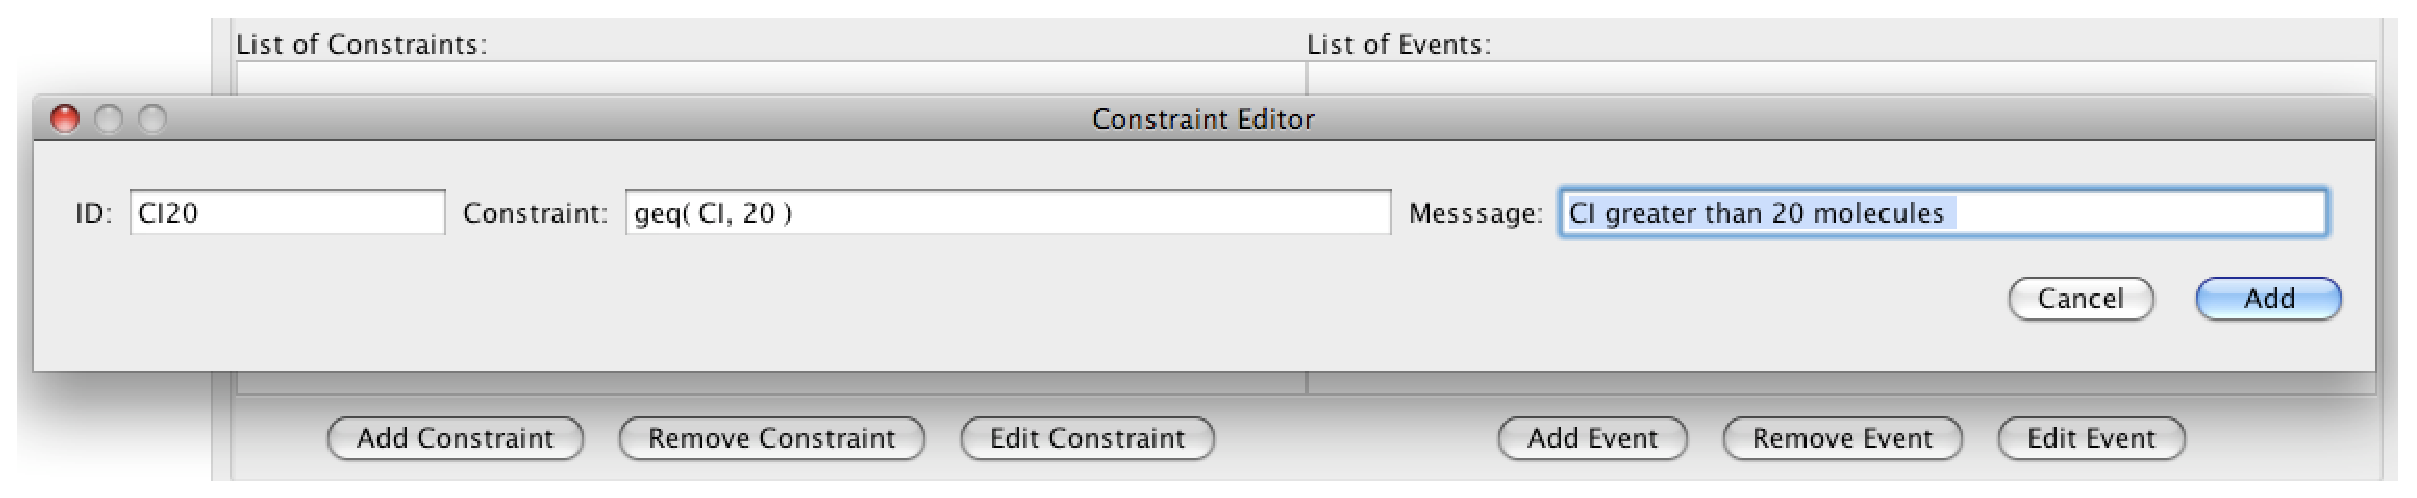
\includegraphics[height=30mm]{screenshots/constraint}

\clearpage

\item Go back to your analysis view by clicking on the {\tt sim} tab.
Remove the simulation ID and press {\tt Save and Run}.  Click on the 
{\tt Probability Graph} tab.
%% 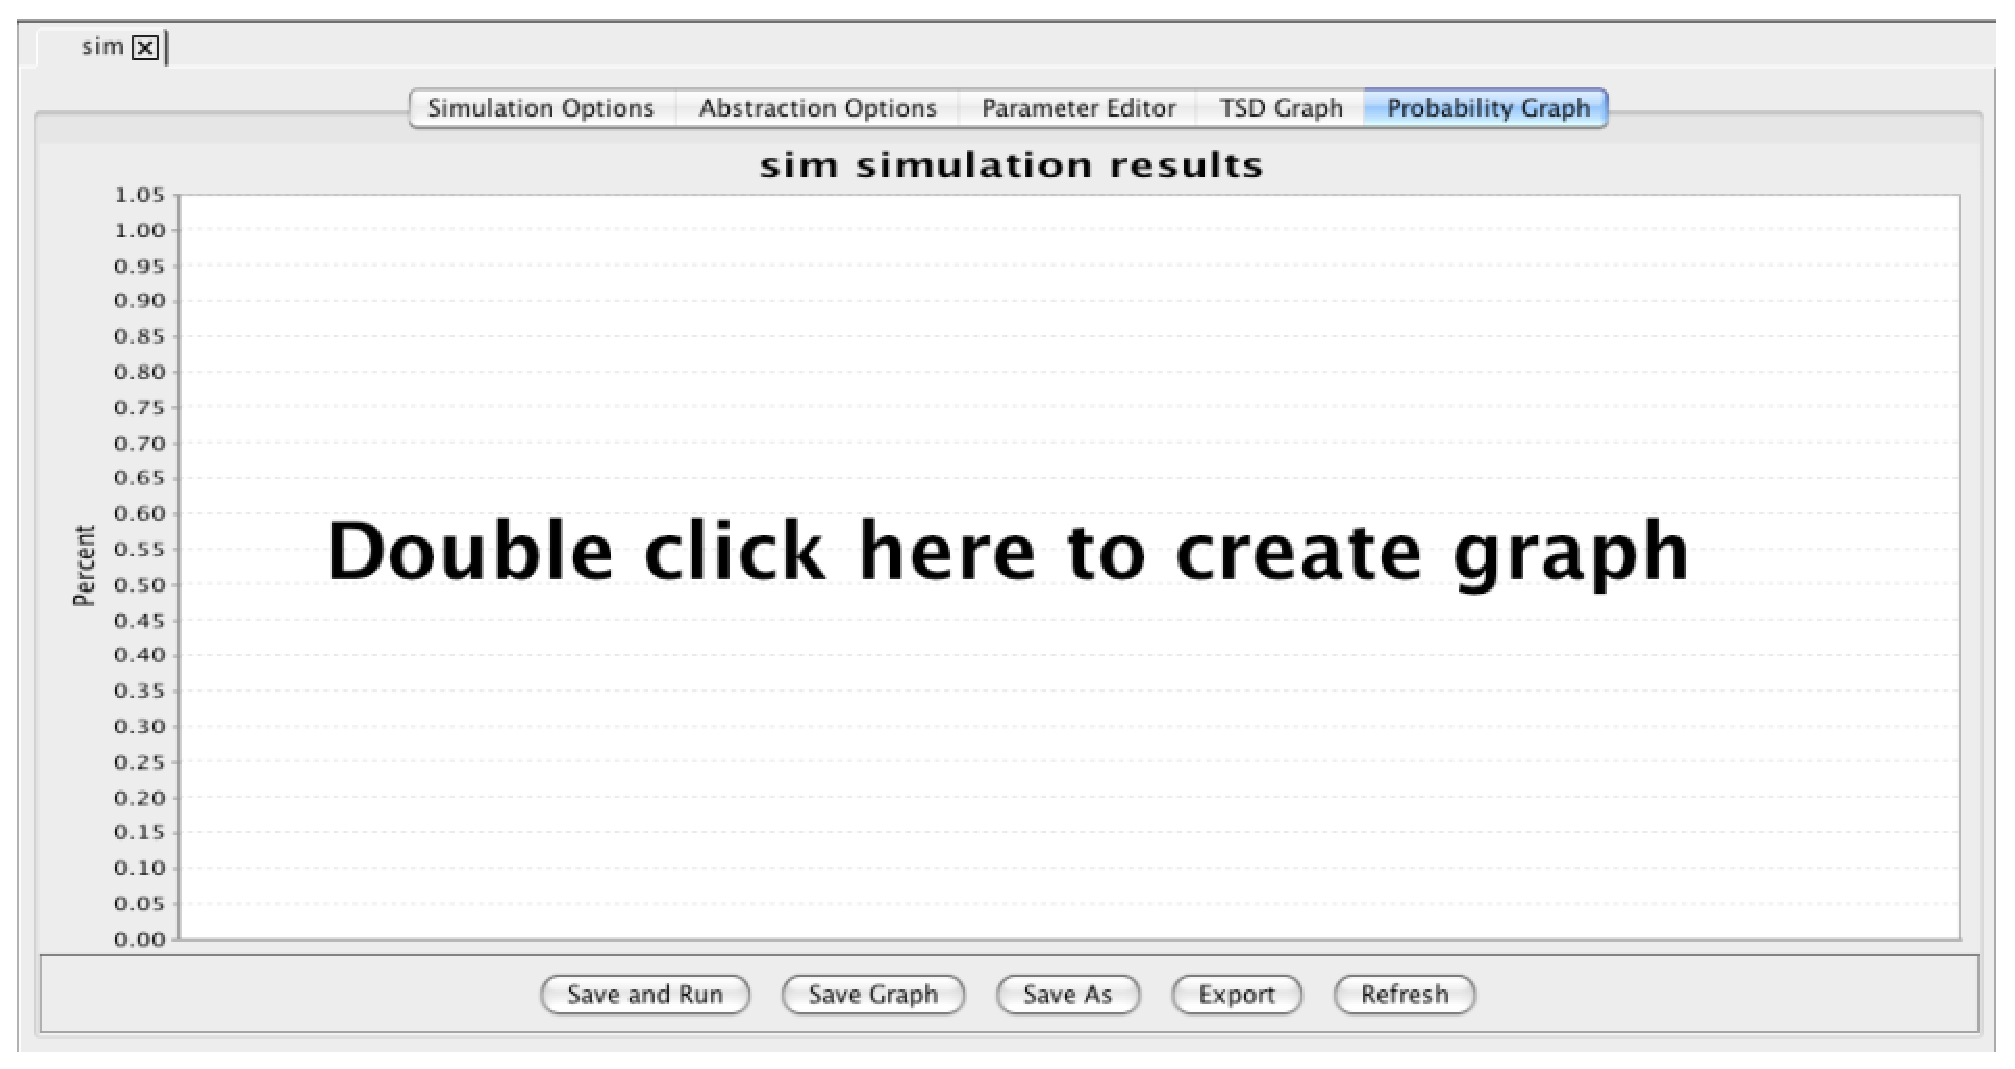
\includegraphics[height=80mm]{screenshots/emptyProbGraph}
%% \item 
Double click on the graph to bring up the probability graph
  editor.  Change the title to {\tt Probability Results} and the 
Y-axis label to {\tt Percent}.  Click on the {\tt sim-rep} file on the 
left-hand side.  Select {\tt CI20}, {\tt CII30}, and {\tt t200} to
graph them.  Press {\tt Ok}.

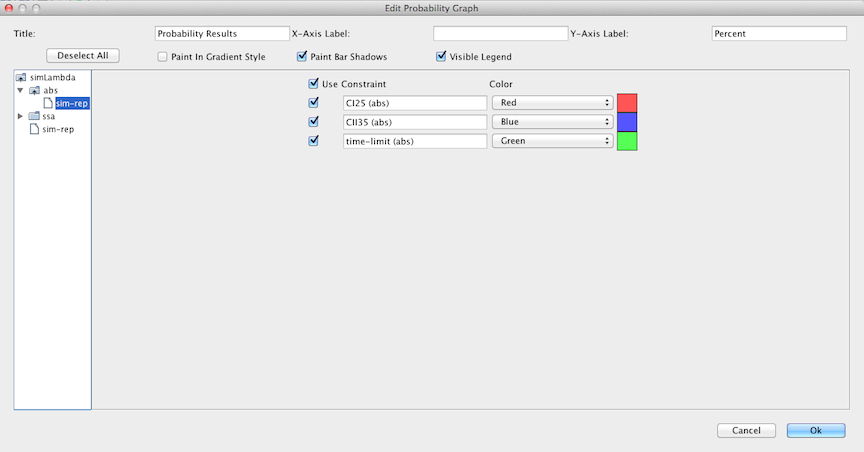
\includegraphics[height=80mm]{screenshots/editProbGraph}

\item Export the graph as a jpg file by selecting the {\tt Export}
  button and entering the filename {\tt prob.jpg}.

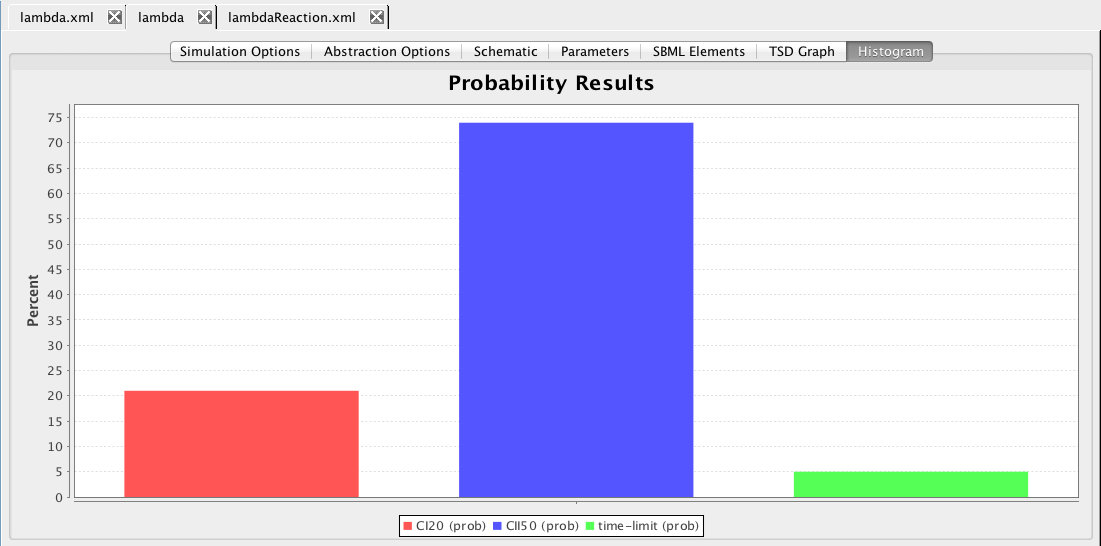
\includegraphics[height=90mm]{screenshots/probResults}

\end{enumerate}

\clearpage

\section{GCM Learning}

This section describes how a GCM can be learned from time series data.
\begin{enumerate}
\item Highlight {\tt CI\_CII.gcm}, right click on it, and select
{\tt Create Learn View}.  Give the learn view the ID {\tt learn}.

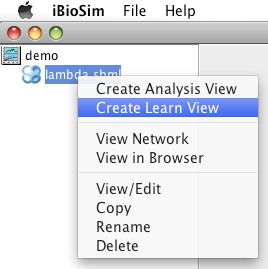
\includegraphics[height=60mm]{screenshots/createLearn}

\item At this point a {\tt Learn View} will open, and you could begin
to add your experimental data.  In this demo, we will just utilize our
simulation data as synthetic experimental data.  To do this, click
{\tt Copy From View}, and select {\tt sim/ssa}.  Highlight 
{\tt sim/ssa/run-1.tsd}, and you should see the simulation data for 
{\tt CI} and {\tt CII} appear on the right in the data editor. 

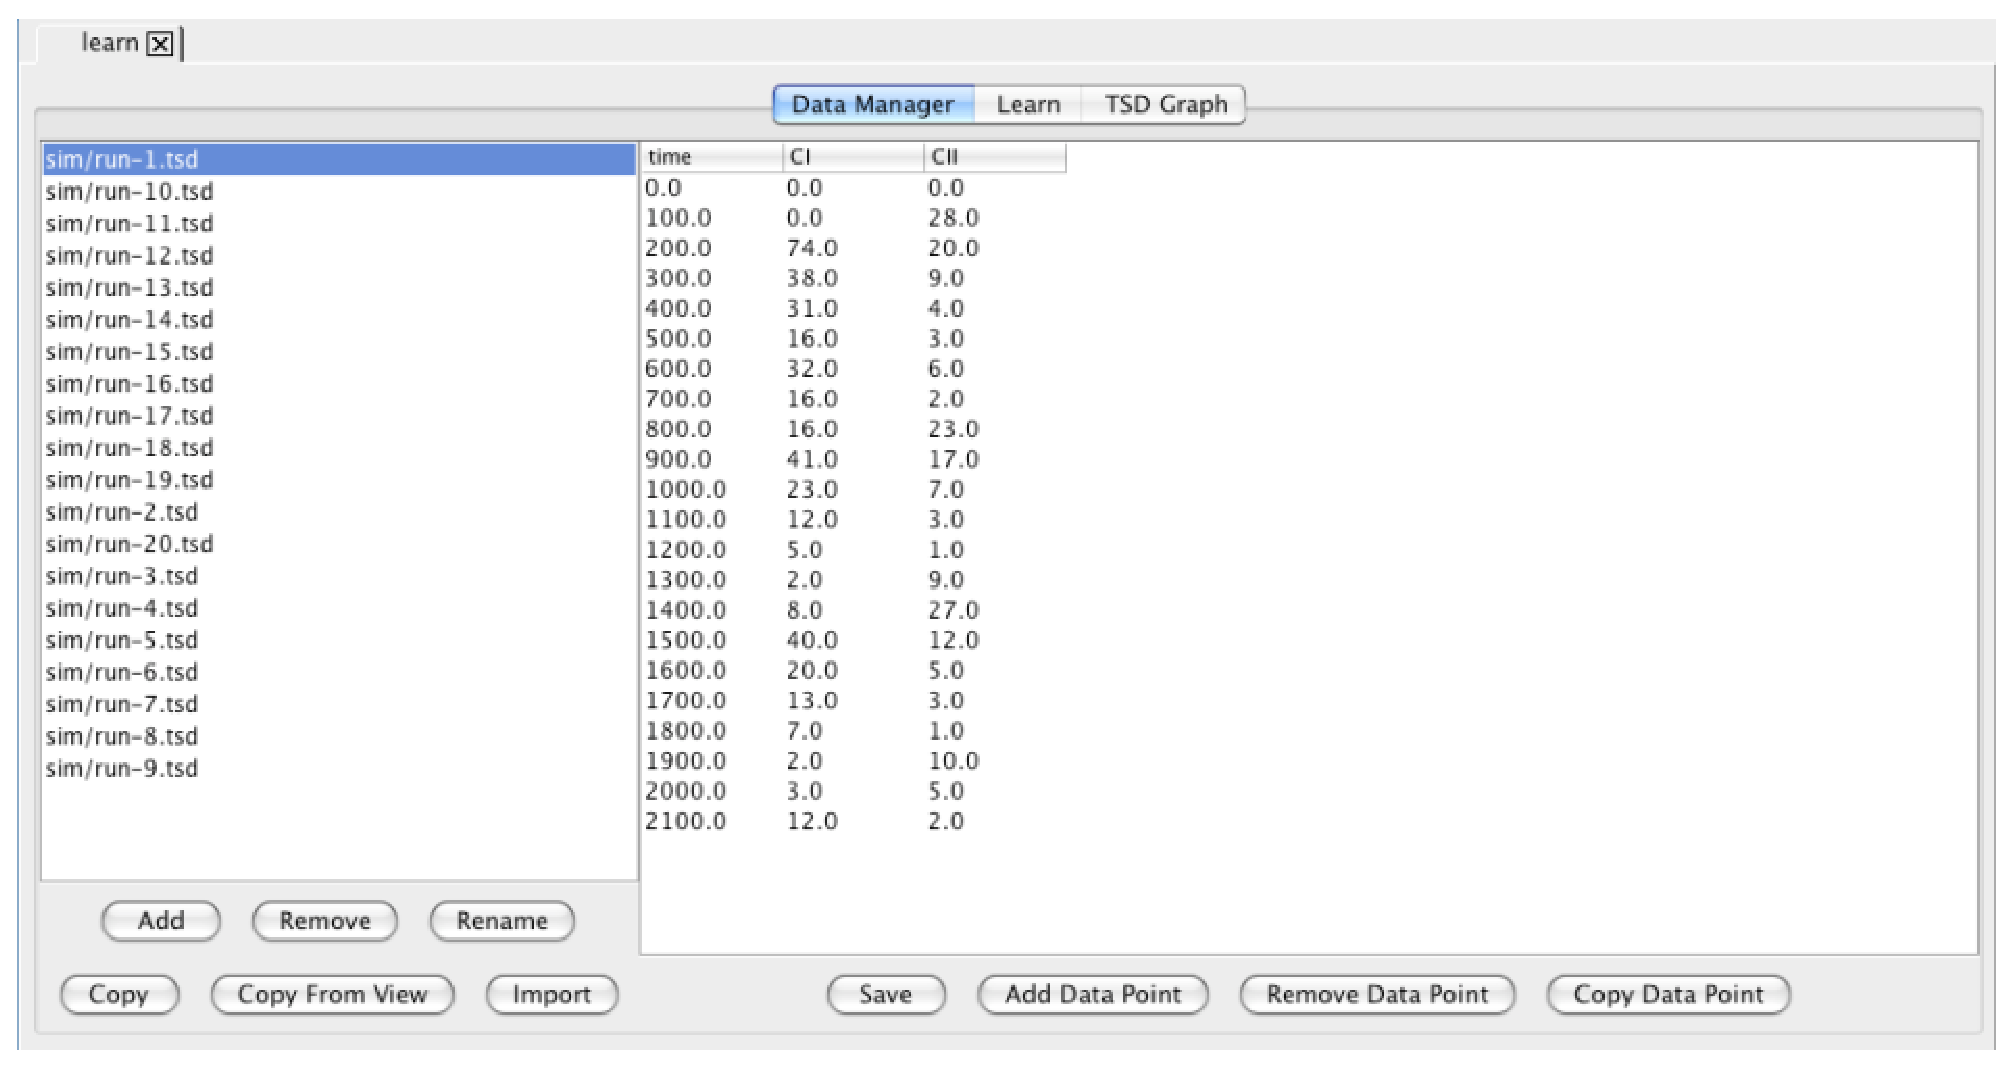
\includegraphics[height=80mm]{screenshots/dataManager}

\clearpage

\item Click on the {\tt Learn} tab.  Here you can edit the various
  learning options.  For example, you can either use auto generated
  levels or user generated levels for your data encoding.  Select 
{\tt Use User Generated Levels} which will make the levels below
editable.  You can also select how many bins to use.  Change the
number of bins for both {\tt CI} and {\tt CII} to 3.  At this point,
you can ask the tool to suggest levels by clicking on the {\tt Suggest
  Levels} button.  Finally, press {\tt Save and Learn} which will
bring up the GCM that has been learned from this experimental data
using Graphviz's dotty program.

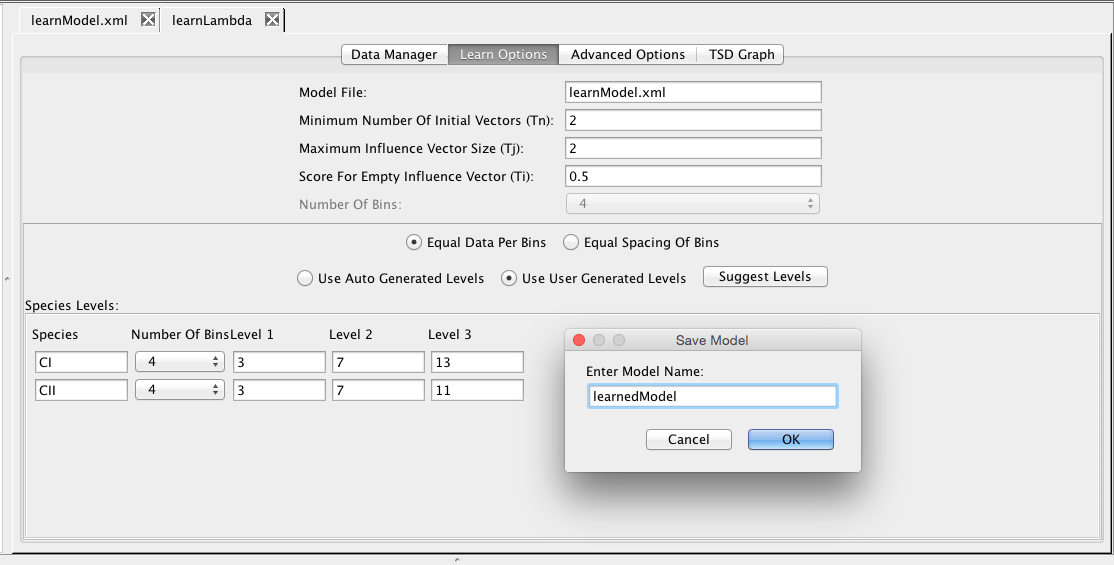
\includegraphics[height=80mm]{screenshots/learn}
\end{enumerate}
 
\clearpage

\section{Genetic Circuit Design}

This last section describes how {\tt iBioSim} can be used to design
genetic logic gates.
\begin{enumerate}
\item Select {\tt File $\rightarrow$ New $\rightarrow$ Genetic Circuit
    Model} and give it the ID {\tt gate}.
\item Add promoters {\tt P1} and {\tt P2}, species {\tt A}, {\tt B},
  and {\tt C} (make {\tt A} and {\tt B} type {\tt boundary} and {\tt
    C} type normal), and repression influences from {\tt A} to {\tt C} on
  {\tt P1} and {\tt B} to {\tt C} on {\tt P2}.  Save as an SBML
  template named {\tt gateEnv}, and associate that SBML file with this
  GCM.  Finally, save the GCM.
\item Open {\tt gateEnv.sbml} in an SBML editor.  Click on the\\ 
      {\tt Initial Assignments/Rules/Constraints/Events} tab, and
      select {\tt Add Event}.
\item In the event editor, give a trigger of {\tt geq(t,2000)}.   
      Press {\tt Add Assignment}, select variable {\tt A}, and enter
      60 in the {\tt Assignment} field.  Press {\tt Add} for the event
      assignment and {\tt Add} for the event.  Repeat these steps to
      create an assignment to {\tt B} of 60 at time 4000.  Note that
      you may ignore the warnings.  These can be suppressed by
      changing your preferences and deselecting {\tt Check for
        undeclared units in SBML}.  Be sure to press {\tt Save SBML}
      when you are done.
\item Highlight {\tt gate.gcm}, right-click, and select {\tt Create
    Analysis View}.  Give it the ID {\tt simGate}.
\item In the analysis view, change the options to 
      {\tt Monte Carlo}, time limit of 6000, print interval of 30,
      runs of 100.  
%% Click on the {\tt Abstractions Options} tab.
%%      Highlight {\tt A} and press {\tt Add Species}.  Repeat for {\tt
%%        B} and {\tt C} to also make them interesting species.
      Press {\tt Save and Run}.
\item Select the {\tt TSD Graph} tab and graph the averages of {\tt
    A},  {\tt B}, and {\tt C}.  The behavior should be that of a Nand
  gate.

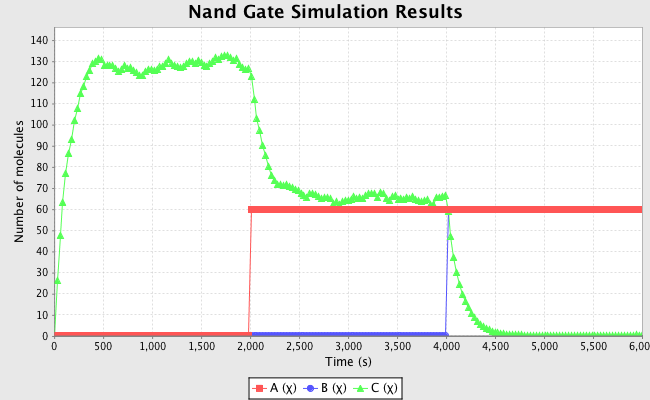
\includegraphics[height=90mm]{screenshots/nandResults}

\clearpage

\item Go back to the GCM editor for {\tt gate}.  Change the promoter
  on the influence from {\tt B} to {\tt C} to {\tt P1}, and save the
  GCM.  Go back to your analysis view and press {\tt Save and Run}.
  The behavior should now be that of a Nor gate.

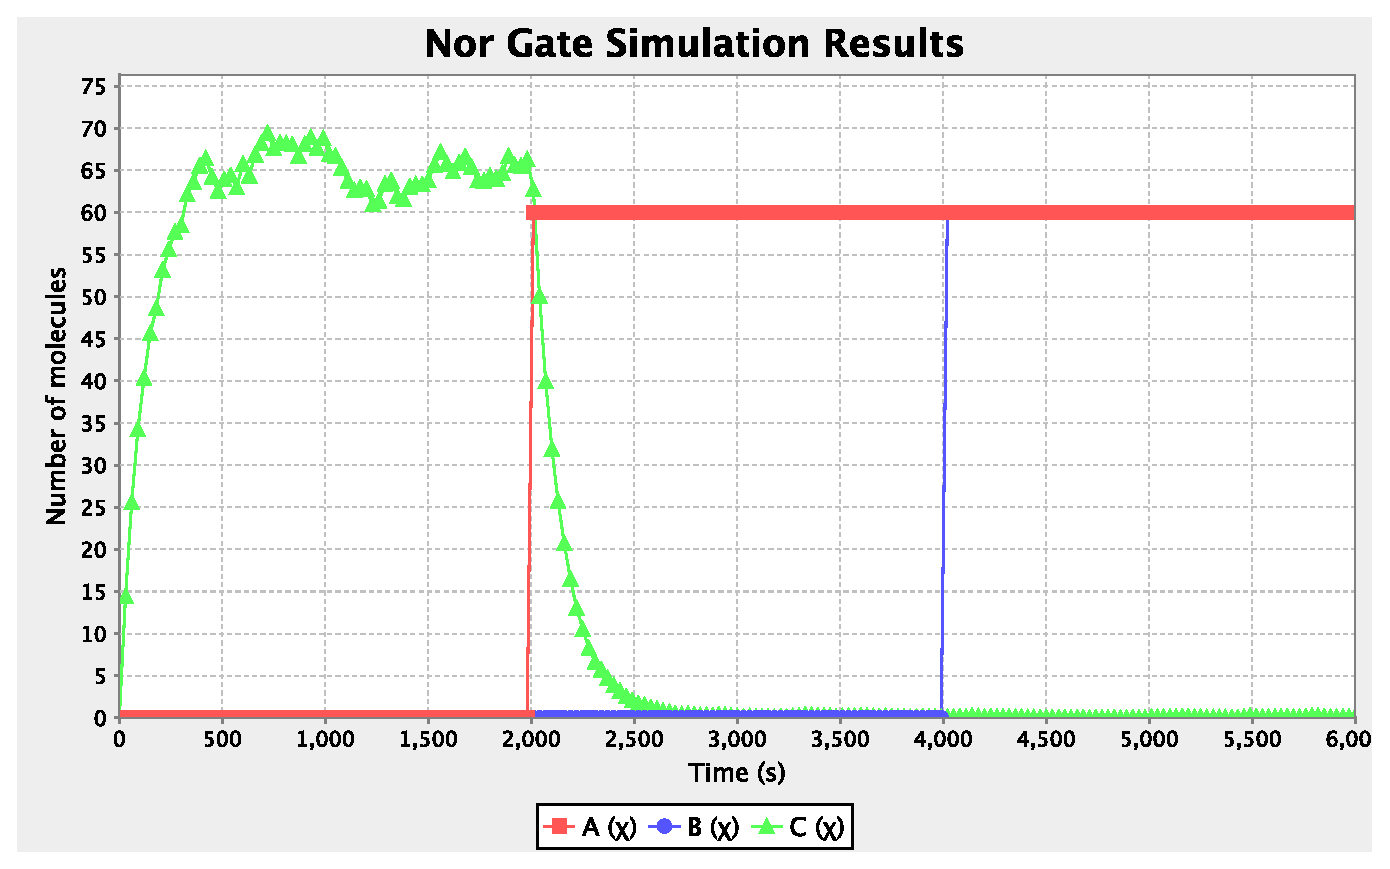
\includegraphics[height=90mm]{screenshots/norResults}

\end{enumerate}
  
\end{document}
